%Version 3.1 December 2024
% See section 11 of the User Manual for version history
%
%%%%%%%%%%%%%%%%%%%%%%%%%%%%%%%%%%%%%%%%%%%%%%%%%%%%%%%%%%%%%%%%%%%%%%
%%                                                                 %%
%% Please do not use \input{...} to include other tex files.       %%
%% Submit your LaTeX manuscript as one .tex document.              %%
%%                                                                 %%
%% All additional figures and files should be attached             %%
%% separately and not embedded in the \TeX\ document itself.       %%
%%                                                                 %%
%%%%%%%%%%%%%%%%%%%%%%%%%%%%%%%%%%%%%%%%%%%%%%%%%%%%%%%%%%%%%%%%%%%%%

%%\documentclass[referee,sn-basic]{sn-jnl}% referee option is meant for double line spacing

%%=======================================================%%
%% to print line numbers in the margin use lineno option %%
%%=======================================================%%

%%\documentclass[lineno,pdflatex,sn-basic]{sn-jnl}% Basic Springer Nature Reference Style/Chemistry Reference Style

%%=========================================================================================%%
%% the documentclass is set to pdflatex as default. You can delete it if not appropriate.  %%
%%=========================================================================================%%

%%\documentclass[sn-basic]{sn-jnl}% Basic Springer Nature Reference Style/Chemistry Reference Style

%%Note: the following reference styles support Namedate and Numbered referencing. By default the style follows the most common style. To switch between the options you can add or remove “Numbered” in the optional parenthesis. 
%%The option is available for: sn-basic.bst, sn-chicago.bst%  
 
%%\documentclass[pdflatex,sn-nature]{sn-jnl}% Style for submissions to Nature Portfolio journals
%%\documentclass[pdflatex,sn-basic]{sn-jnl}% Basic Springer Nature Reference Style/Chemistry Reference Style
\documentclass[pdflatex,sn-mathphys-num]{sn-jnl}% Math and Physical Sciences Numbered Reference Style
%%\documentclass[pdflatex,sn-mathphys-ay]{sn-jnl}% Math and Physical Sciences Author Year Reference Style
%%\documentclass[pdflatex,sn-aps]{sn-jnl}% American Physical Society (APS) Reference Style
%%\documentclass[pdflatex,sn-vancouver-num]{sn-jnl}% Vancouver Numbered Reference Style
%%\documentclass[pdflatex,sn-vancouver-ay]{sn-jnl}% Vancouver Author Year Reference Style
%%\documentclass[pdflatex,sn-apa]{sn-jnl}% APA Reference Style
%%\documentclass[pdflatex,sn-chicago]{sn-jnl}% Chicago-based Humanities Reference Style

%%%% Standard Packages
%%<additional latex packages if required can be included here>
\usepackage{rotating}
\usepackage{graphicx}%
\usepackage{multirow}%
\usepackage{amsmath,amssymb,amsfonts}%
\usepackage{amsthm}%
\usepackage{mathrsfs}%
\usepackage[title]{appendix}%
\usepackage{xcolor}%
\usepackage{textcomp}%
\usepackage{manyfoot}%
\usepackage{booktabs}%
\usepackage{placeins}%
\usepackage{algorithm}%
\usepackage{algorithmicx}%
\usepackage{algpseudocode}%
\usepackage{listings}%
%%%%
\usepackage[T1]{fontenc} 
%%%%%=============================================================================%%%%
%%%%  Remarks: This template is provided to aid authors with the preparation
%%%%  of original research articles intended for submission to journals published 
%%%%  by Springer Nature. The guidance has been prepared in partnership with 
%%%%  production teams to conform to Springer Nature technical requirements. 
%%%%  Editorial and presentation requirements differ among journal portfolios and 
%%%%  research disciplines. You may find sections in this template are irrelevant 
%%%%  to your work and are empowered to omit any such section if allowed by the 
%%%%  journal you intend to submit to. The submission guidelines and policies 
%%%%  of the journal take precedence. A detailed User Manual is available in the 
%%%%  template package for technical guidance.
%%%%%=============================================================================%%%%

%% as per the requirement new theorem styles can be included as shown below
\theoremstyle{thmstyleone}%
\newtheorem{theorem}{Theorem}%  meant for continuous numbers
%%\newtheorem{theorem}{Theorem}[section]% meant for sectionwise numbers
%% optional argument [theorem] produces theorem numbering sequence instead of independent numbers for Proposition
\newtheorem{proposition}[theorem]{Proposition}% 
%%\newtheorem{proposition}{Proposition}% to get separate numbers for theorem and proposition etc.

\theoremstyle{thmstyletwo}%
\newtheorem{example}{Example}%
\newtheorem{remark}{Remark}%

\theoremstyle{thmstylethree}%
\newtheorem{definition}{Definition}%

\raggedbottom
%%\unnumbered% uncomment this for unnumbered level heads

\begin{document}

\title{MTTravel-Bench: A Dynamic Narrative Benchmark for Evaluating Mental-Time-Travel Option Reasoning and Factual Foresight in Large Language Models}
%%=============================================================%%
%% GivenName	-> \fnm{Joergen W.}
%% Particle	-> \spfx{van der} -> surname prefix
%% FamilyName	-> \sur{Ploeg}
%% Suffix	-> \sfx{IV}
%% \author*[1,2]{\fnm{Joergen W.} \spfx{van der} \sur{Ploeg} 
%%  \sfx{IV}}\email{iauthor@gmail.com}
%%=============================================================%%

\author[1,2,3]{\fnm{Qing} \sur{Li}}\email{tsinglee@ieee.org}

\author[1]{\fnm{Qian} \sur{Fu}}\email{fuqian.gdxlzxzx@gmail.com}
% \equalcont{These authors contributed equally to this work.}

\author*[1,2,3]{\fnm{Yongbin} \sur{Qin}}\email{ybqin@gzu.edu.cn}

\affil[1]{\orgdiv{Guizhou Provincial Laboratory of Big Data, State Key Laboratory of Public Big Data}, \orgname{Guizhou University}, \orgaddress{\city{Guiyang}, \postcode{550025}, \state{Guizhou}, \country{China}}}

\affil[2]{\orgdiv{College of Computer Science and Technology}, \orgname{Guizhou University}, \orgaddress{ \city{Guiyang}, \postcode{550025}, \state{Guizhou}, \country{China}}}

\affil*[3]{\orgdiv{Text Computing and Cognitive Intelligence Engineering Research Center of National Education Ministry}, \orgname{Guizhou University}, \orgaddress{ \city{Guiyang}, \postcode{550025}, \state{Guizhou}, \country{China}}}

%%==================================%%
%% Sample for unstructured abstract %%
%%==================================%%

\abstract{In recent years, the evaluation of large language models has been shifting from static question-answering tasks toward dynamic behavioral assessment. However, existing evaluations still rely on short texts or isolated tasks, and therefore lack a set of characterization of how models perform action reasoning in continuous contexts. In particular, they provide limited evidence on whether models can integrate past experience, current states, and future consequences during decision-making based reasoning. The theory of mental time travel in cognitive science provides a core construct for understanding this capacity. It describes the ability of individuals to reconstruct past experiences, project the self into possible future situations, and maintain self-continuity across time. To introduce this construct into the evaluation of large language models, this paper proposes MTTravel-Bench, a dynamic narrative benchmark that operationalizes mental time travel as an NLP evaluation task. MTTravel-Bench is constructed from TellMeWhy, NTSB aviation accident reports, and FairytaleQA, covering everyday causal narratives, real-world accident narratives, and fictional long-range narratives. It transforms narrative episodes into reasoning nodes centered trajectories and represents event order, causal dependencies, and reachable future paths using directed acyclic graphs. At each decision node, the benchmark generates temporally grounded action options and maps them onto three dimensions of mental time travel: spatiotemporal reconstruction, self-projection, and self-state consistency. It also identifies factual options that follow the original narrative trajectory, enabling the evaluation of models' ability to predict subsequent factual outcomes. MTTravel-Bench evaluates action reasoning through two complementary tasks defined at the same narrative causal graph nodes. Task1 profiles utility-implied action orientation across factual and diagnostic actions, while Task2 measures models' ability to predict the structured consequences of factual actions. Evaluating both capabilities within the same causal--temporal context enables fine-grained diagnosis of action assessment and consequence prediction. Experiments with 30 models on 4,453 shared casual graph nodes show that the benchmark distinguishes model behavior across task dimensions and narrative domains. MTTravel-Bench therefore provides a scalable, cross-domain framework for analyzing how LLMs use prior narrative states and current decision constraints to reason about future outcomes.}

%%================================%%
%% Sample for structured abstract %%
%%================================%%

% \abstract{\textbf{Purpose:} The abstract serves both as a general introduction to the topic and as a brief, non-technical summary of the main results and their implications. The abstract must not include subheadings (unless expressly permitted in the journal's Instructions to Authors), equations or citations. As a guide the abstract should not exceed 200 words. Most journals do not set a hard limit however authors are advised to check the author instructions for the journal they are submitting to.
% 
% \textbf{Methods:} The abstract serves both as a general introduction to the topic and as a brief, non-technical summary of the main results and their implications. The abstract must not include subheadings (unless expressly permitted in the journal's Instructions to Authors), equations or citations. As a guide the abstract should not exceed 200 words. Most journals do not set a hard limit however authors are advised to check the author instructions for the journal they are submitting to.
% 
% \textbf{Results:} The abstract serves both as a general introduction to the topic and as a brief, non-technical summary of the main results and their implications. The abstract must not include subheadings (unless expressly permitted in the journal's Instructions to Authors), equations or citations. As a guide the abstract should not exceed 200 words. Most journals do not set a hard limit however authors are advised to check the author instructions for the journal they are submitting to.
% 
% \textbf{Conclusion:} The abstract serves both as a general introduction to the topic and as a brief, non-technical summary of the main results and their implications. The abstract must not include subheadings (unless expressly permitted in the journal's Instructions to Authors), equations or citations. As a guide the abstract should not exceed 200 words. Most journals do not set a hard limit however authors are advised to check the author instructions for the journal they are submitting to.}

\keywords{large language models; dynamic benchmark; directed acyclic graph; AI agent evaluation.}

%%\pacs[JEL Classification]{D8, H51}

%%\pacs[MSC Classification]{35A01, 65L10, 65L12, 65L20, 65L70}

\maketitle

\section{Introduction}\label{sec1}

Large language models (LLMs) have rapidly developed from general-purpose text generators into systems that support work across education, software development, and scientific research \cite{zhao2023survey,kasneci2023chatgpt,peng2023impact,noy2023experimental,boiko2023autonomous}. Beyond open-domain question answering, general-purpose models have achieved strong results on professional and academic assessments originally designed for human test takers \cite{openai2023gpt4}. Recent benchmarks have raised the standard further by testing research-level mathematics and expert knowledge across a broad range of academic fields \cite{glazer2024frontiermath,hle2026benchmark}. Together, these advances point to the growing potential of general-purpose LLMs as tools for complex intellectual and operational tasks. They also make rigorous evaluation increasingly important, particularly when models must reason over changing states, available actions, and their consequences.

Most benchmarks for large language models assess task performance on standardized, independent instances \cite{srivastava2022beyond}. MMLU, for example, evaluates models across academic and professional domains using separate question-answering items \cite{hendrycks2020measuring}. More recent holistic frameworks, such as HELM, extend this approach to additional scenarios, metrics, and model behaviors \cite{liang2022holistic}. However, they generally retain predefined task instances as the unit of evaluation, with each response scored independently of the model's prior actions. This setup has made model comparisons more systematic and improved the measurement of general language model capabilities. It also assumes that capability can be represented as a fixed input--output mapping evaluated one instance at a time. Such evaluation does not capture how prior actions, accumulated experience, or changing states shape later decisions.

Recent work has moved beyond static benchmarks by treating LLMs as agents that operate under environmental constraints, rather than solely as systems that generate answers. General agent benchmarks assess reasoning, planning, and decision-making based reasoning across multiple interactive environments and task settings. AgentBench, for example, evaluates LLM agents across varied interactive scenarios, with reasoning and decision-making based reasoning in complex environments as its main targets \cite{liu2023agentbench}. Other benchmarks impose more realistic operational constraints, requiring agents to complete long-horizon tasks through direct interactions with external systems. WebArena provides functional web environments in which agents translate high-level natural-language goals into multi-step actions over websites and information resources \cite{zhou2023webarena}. It therefore evaluates task execution under realistic interactive conditions. These benchmarks shift the focus from accuracy on static tasks to the ability to act effectively in interactive environments. However, they do not fully address whether an agent can use prior narrative state or distinguish structurally different action alternatives. They also leave open whether the agent can anticipate the downstream consequences of a specified action within an extended causal--temporal trajectory.

The cognitive motivation for this benchmark draws on research into future-oriented cognition. Early accounts of episodic future thinking described imagining personally relevant future events as a projection of the self into the future, rather than a simple extension of semantic knowledge \cite{atance2001episodic}. Research on mental time travel and foresight further linked this capacity to autobiographical memory, treating both as related abilities that support anticipatory behavior \cite{suddendorf2007evolution}. Constructive episodic simulation offers a related account in which episodic memory is more than a passive record of past events. Details from previous experiences can be selectively retrieved and flexibly recombined to simulate possible futures \cite{schacter2007cognitive}. Subsequent studies have clarified the cognitive and neural mechanisms of episodic future thinking, together with its functional roles \cite{schacter2017episodic}. Work on prospection has also situated episodic simulation within a broader family of future-oriented processes, including prediction, planning, intention, and evaluation \cite{szpunar2014taxonomy}.

This body of research provides the conceptual motivation for our benchmark, we reformulate future-oriented cognition as a well-defined and computationally tractable task framework. Specifically, we examine whether an LLM can represent alternative actions and predict the consequences of factual actions within a dynamic narrative trajectory. The central question is whether LLMs can use prior narrative state to distinguish between structurally different candidate actions. We also ask whether the model can infer consistent and plausible consequences of a specified action under the story's causal and temporal constraints.

Related benchmarks address different parts of this problem through forecasting, temporal reasoning, and long-term memory. Forecasting benchmarks test whether AI systems can produce well-calibrated probabilistic predictions about future events under changing evaluation distributions. ForecastBench, for example, is continuously updated to measure forecasting accuracy on future-oriented queries \cite{karger2024forecastbench}. Temporal reasoning benchmarks instead isolate models' ability to process temporal relations, logic, and arithmetic under controlled conditions. Test of Time uses synthetic datasets to evaluate LLMs across a range of temporal reasoning tasks while limiting data leakage from real-world corpora \cite{fatemi2024test}. Work on long-term memory focuses on interactive systems, asking whether conversational agents can retrieve, update, and reason over information distributed across extended multi-turn histories. LongMemEval evaluates information extraction, cross-session reasoning, temporal reasoning, knowledge updating, and abstention in long-horizon interactions \cite{wu2024longmemeval}.

These benchmarks have improved the evaluation of future-oriented prediction, temporal inference, and long-context retrieval. However, they do not bring action alternatives, local causal dependencies, and factual trajectory continuation together within a single evaluation instance. Forecasting benchmarks generally test predictions about future events, not the downstream consequences of a specified action within a structured narrative trajectory. Temporal reasoning benchmarks test time-sensitive inference but rarely require comparisons among alternative actions under explicit local causal constraints. Long-term memory benchmarks examine whether models can retrieve and use historical context across extended interactions. They do not test whether an action selected at a decision node leads to a causally consistent factual continuation. Failures under existing protocols therefore remain difficult to diagnose. A model may misinterpret the options, lose track of the narrative state, violate causal--temporal constraints, or hallucinate an outcome.

Our benchmark is also motivated by recent work on benchmark validity and evaluation science. This literature treats benchmarks not simply as collections of test items, but as measurement instruments. Their scores are meaningful only when the target construct, task design, scoring procedure, and intended interpretation are aligned. Wallach et al.\ frame generative AI evaluation as a measurement problem. They argue that evaluation should begin by defining the target capability or behavior and explaining how task performance provides evidence for it \cite{wallach2025position}. Bean et al.\ examine LLM benchmarks through the lens of construct validity. They show that benchmark conclusions are weakened when target phenomena are poorly specified, tasks are weakly mapped to them, or metrics do not support the intended interpretation \cite{bean2025measuring}. At the framework level, Weidinger et al.\ identify validity challenges in commonly used static benchmarks. They call for an evaluation science that is transparent, iterative, and more closely tied to real-world deployment contexts \cite{weidinger2025evaluation}. This measurement perspective has a direct implication for our benchmark. Compressing narrative decision competence into one aggregate score makes it difficult to distinguish option understanding, state tracking, causal-constraint use, and consequence prediction.

Recent work on preference heterogeneity and aggregation raises a related concern for AI alignment. Research on pluralistic and personalized alignment shows that human preferences vary across people and contexts. A single reward model or ranking can therefore obscure meaningful differences among user groups and evaluation settings. MaxMin-RLHF formalizes this limitation through an impossibility result showing that no single reward function can represent groups with genuinely different preferences. Its egalitarian MaxMin objective improves minority-group win rates by more than 33\% without reducing majority-group performance \cite{chakraborty2024maxmin}. Work on annotator disagreement similarly shows that majority-vote aggregation can discard genuine judgments from target groups. Modeling individual annotators improved predictions of individual ratings by 22\% and annotator variance by 33\% relative to the reported baseline \cite{fleisig2023when}. By analogy, a benchmark that compresses a multidimensional capability profile into one score may hide systematic differences in how models prioritize reasoning strategies. 

MTTravel-Bench therefore uses a measurement-oriented design that separates narrative decision competence into two evaluation targets. Utility-implied action preference profiling characterizes how a model assigns predicted utility to structurally distinct candidate actions. These estimates are conditioned on the prior narrative state, local causal constraints, and plausible future trajectories. Fact-conditioned consequence prediction measures whether the model can infer the actual subsequent outcome after a specified factual action in the narrative trajectory. This decomposition supports more diagnostic evaluation than an aggregate leaderboard ranking. It helps attribute errors to option misinterpretation, state-tracking failures, violations of causal--temporal constraints, or hallucinated consequences. Recent studies of leaderboard-based evaluation reinforce the need for such diagnostic information. They show that rankings and score differences can be sensitive to selective disclosure, data access, benchmark variance, and unreported uncertainty \cite{singh2025leaderboard,blackwell2024reproducible,madaan2024quantifying}. By analogy with pluralistic alignment, reporting separate capability dimensions preserves meaningful variation that a single summary may obscure \cite{sorensen2024roadmap}.

To address these gaps, we introduce MTTravel-Bench, a benchmark for evaluating how generative language models reason about decisions and consequences in temporally extended narratives. Its design draws on mental time travel as a cognitive construct and translates its functional structure into an AI evaluation problem. Models must use prior narrative context to interpret a present decision, form expectations about possible actions, and predict their consequences. MTTravel-Bench is therefore a measurement framework inspired by cognitive psychology, not a direct psychological test of machine experience. The benchmark draws on TellMeWhy, NTSB aviation accident reports, and FairytaleQA, spanning everyday causal narratives, real-world accidents, and fictional long-horizon stories. Its construction pipeline converts each narrative into a directed acyclic graph that encodes event order, causal dependencies, decision nodes, and reachable future paths. At each decision node, it generates temporally grounded candidate actions. Diagnostic actions correspond to spatiotemporal reconstruction, self-projection, and self-state consistency, while the factual action follows the original narrative trajectory. Two complementary measurements are applied to every node. Utility-implied action preference profiling records how a model distributes predicted utility across factual and diagnostic action types without imposing a gold preference label. Fact-conditioned consequence prediction tests whether the model can recover the structured consequences and fine-grained local outcomes that follow the factual action. This design provides a reusable narrative-to-graph construction method and a diagnostic framework that separates action preference from consequence prediction. Experiments with 30 models on a shared set of 4,453 decision nodes show that the two measurements are related but capture distinct, domain-sensitive aspects of model behavior. The resulting benchmark supports cross-domain analysis of how models interpret actions, maintain narrative state, and reason about causally constrained futures.

Figure~\ref{fig:measurement-case} illustrates how this framework is applied to a representative MTTravel-Bench measurement case. The model receives a narrative episode that ends at a key decision point, together with the preceding context and several visible candidate actions. The first measurement tests whether the model can estimate a structural profile for each candidate action. It considers whether the action requires reconstructing earlier temporal and causal information or projecting the future state of the actor or another relevant subject. The profile also captures consistency with the preceding trajectory and the action's local utility. Because no option type is normatively correct, the benchmark reports these predictions as a descriptive utility-implied action preference profile rather than scoring them against a gold label. The second measurement fixes the factual action and asks the model to predict the consequence structure that follows. Together, these measurements capture utility-implied action preference profiling and fact-conditioned consequence prediction within a single decision-node instance.

\begin{figure}[htbp]
\centering
    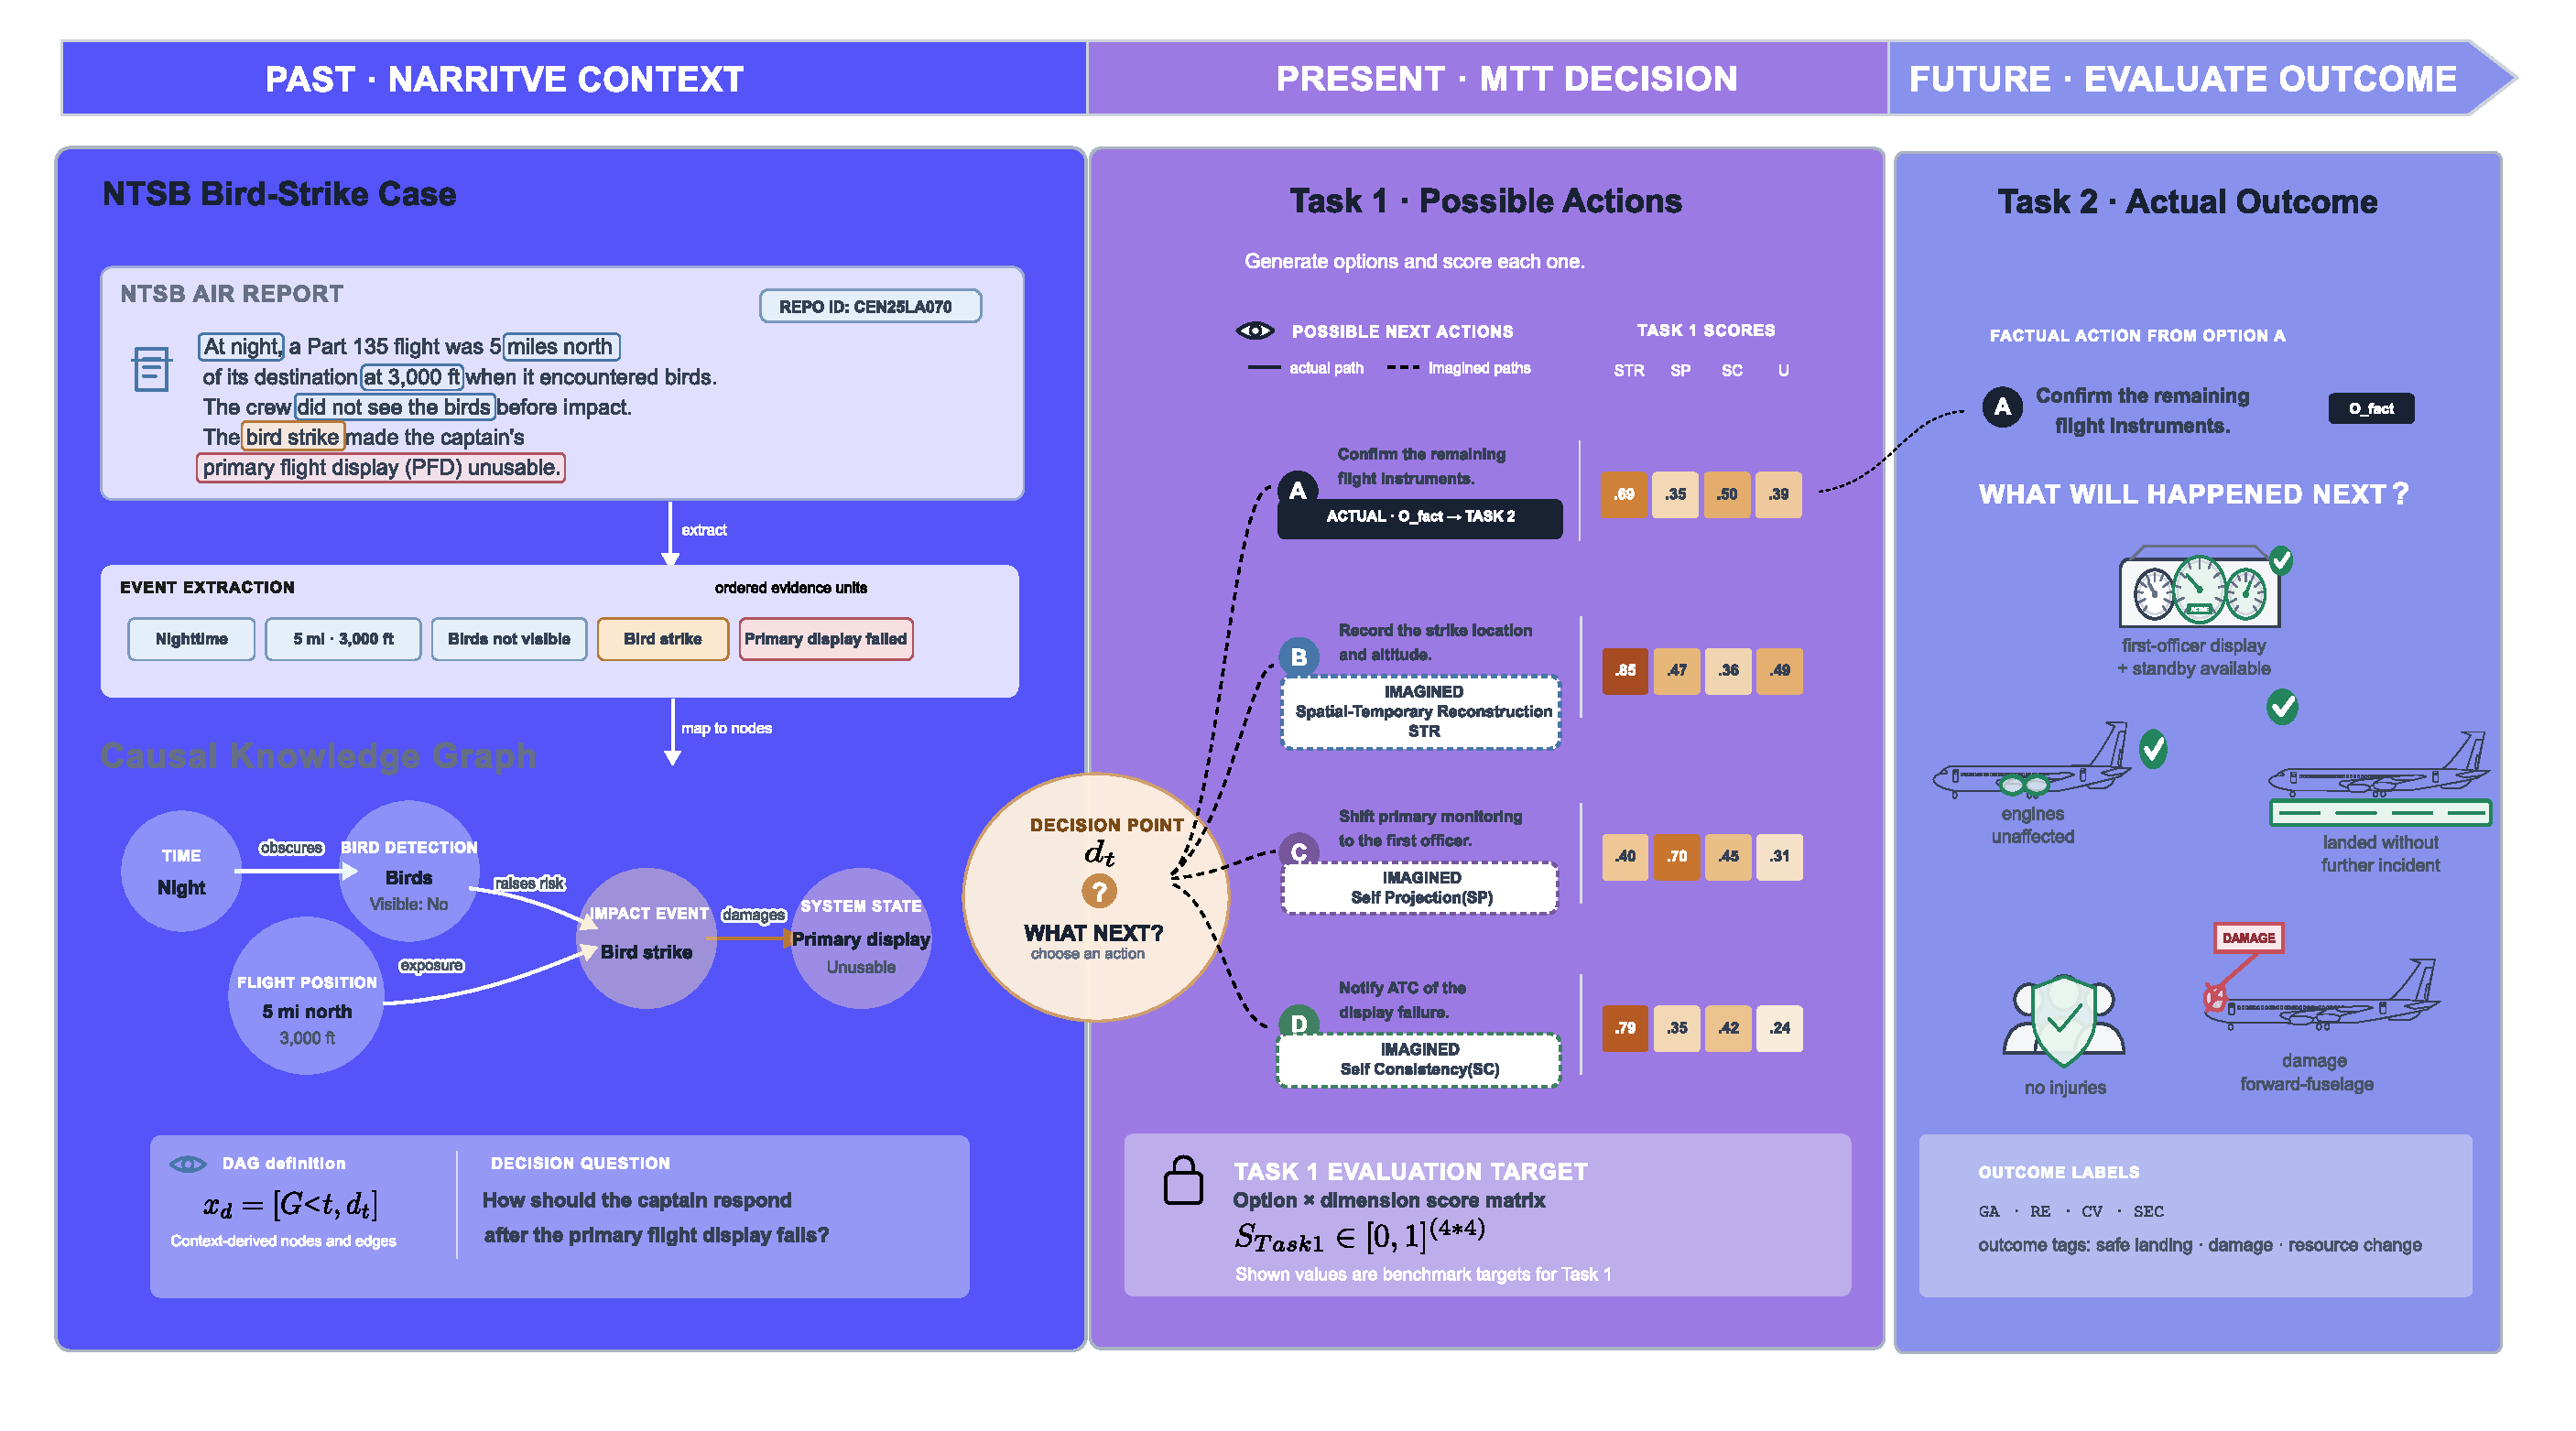
\includegraphics[width=1\linewidth]{mttravel_figure1_measurement_case.pdf}
\caption{A measurement case in MTTravel-Bench. The model receives a prior narrative context and candidate actions at a key decision node. The benchmark measures candidate-action structural expectations and fact-conditioned consequence prediction.}
\label{fig:measurement-case}
\end{figure}
A key feature of MTTravel-Bench is its use of existing narrative materials instead of manually authored interactive environments. The benchmark converts public narrative sources into causal--temporal structures that preserve states, actions, constraints, and observable consequences. This allows stories, accident reports, and everyday causal accounts to serve as decision-centered evaluation material. The full construction procedure is described in detail in the \hyperref[sec3]{Materials and Methods section}. The key point is that available narrative evidence becomes measurable instances of decisions and their consequences.

This work makes four contributions.
The first contribution is a reusable construction pipeline that transforms heterogeneous narrative sources into decision-centered causal--temporal directed acyclic graphs (DAGs). It preserves event order, local causal dependencies, factual actions, and reachable consequences. Because the pipeline draws on existing narrative materials, it supports scalable benchmark construction without requiring manually authored interactive environments.
The second contribution is a measurement design that applies two complementary tasks to the same decision nodes. Task~1 uses utility-implied action preference profiling to characterize factual continuation, spatiotemporal reconstruction, self-projection, and self-state and trajectory consistency. Task~2 evaluates fact-conditioned consequence prediction through structured consequence labels, local outcome tags, and exact consistency. Together, these measurements distinguish how models assess candidate actions from how accurately they predict the consequences of a specified action.
The third contribution is a cross-domain benchmark covering everyday causal accounts, high-stakes accident reports, and fictional long-horizon narratives. A common representation and evaluation protocol enables controlled analysis of domain sensitivity and cross-domain stability.
The fourth contribution is a large-scale empirical study of 30 models across 4,453 shared decision nodes. The results demonstrate the framework's diagnostic value by revealing substantial differences across models, measurements, and narrative domains. They also show how action orientation and factual foresight provide complementary views of model behavior.
Together, these contributions provide a general framework for studying how language models connect prior narrative states, current action constraints, and future outcomes. The DAG backbone and reporting protocol can also support future evaluation of branching narratives and memory- or planning-augmented agents.

\section{Related Works}
Work relevant to dynamic narrative decision-making based reasoning can be organized by the increasing scope of behavior under evaluation. Temporal-reasoning and memory benchmarks examine whether models can recover, organize, and retain information across time. Agent benchmarks extend this setting by requiring models to plan and act over multiple steps in interactive environments. Trajectory-level and human-comparable evaluations broaden the scope further by examining complete behavioral sequences under increasingly realistic conditions. Together, these lines of research have established the foundations for evaluating LLMs beyond static question answering. However, action selection, memory use, temporal inference, and consequence prediction are usually assessed in separate settings. MTTravel-Bench brings these capabilities together at narrative decision nodes, where models interpret candidate actions from prior context and predict the factual consequences that follow.

Table\ref{tab:related-work-map} provides an overview of the literature reviewed in this section. It groups representative studies by evaluation setting and mechanism, identifies the primary capability examined by each line of work, and clarifies how MTTravel-Bench differs from existing approaches.

\begin{sidewaystable}[htbp]
\centering
\scriptsize
\caption{Taxonomy of related work. Each row corresponds to a subsection and compares representative methods, primary research targets, and the distinctive focus of MTTravel-Bench.}
\label{tab:related-work-map}
\begin{tabular}{p{0.15\textwidth} p{0.30\textwidth} p{0.23\textwidth} p{0.25\textwidth}}
\toprule
Related-work subsection & Representative categories and studies & Primary research target & Distinctive focus of MTTravel-Bench \\
\midrule
Interactive and Long-Horizon Agent Benchmarks & Text-based environments \cite{cote2018textworld,hausknecht2019interactive,shridhar2020alfworld}; web environments \cite{yao2022webshop,deng2023mind2web,zhou2023webarena}; general and operational environments \cite{liu2023agentbench,xie2024osworld,trivedi2024appworld,yao2024bench,lu2024toolsandbox,xu2024theagentcompany} & Sequential interaction, task execution, and final-state correctness in external environments & Decision-node analysis of candidate actions and factual consequences \\
\midrule
From Static to Dynamic Evaluation & Benchmark validity analysis \cite{bowman2021take}; human--model-in-the-loop data collection \cite{kiela2021dynabench}; generated and difficulty-controlled probing \cite{hu2025dynacode,zhu2024dynamic} & Adaptive test construction, changing data distributions, and difficulty-controlled evaluation & Dynamic causal--temporal structures with linked states and reachable outcomes \\
\midrule
Temporal Reasoning and Future-Event Forecasting & Controlled temporal reasoning \cite{fatemi2024test,uddin2024unseentimeqa}; timeline-based reasoning \cite{tan2023timelineqa,wei2025time}; open-world forecasting \cite{zou2022forecasting,karger2024forecastbench,halawi2024approaching} & Temporal relations, event ordering, and predictions of unresolved future events & Action-conditioned prediction within known local narrative trajectories \\
\midrule
Long-Term Memory Evaluation and Memory-Augmented Agents & Long-term memory benchmarks \cite{wu2024longmemeval,hu2025evaluating}; context management and reflection \cite{packer2023memgpt,shinn2023reflexion}; social and embodied experience reuse \cite{park2023generative,wang2023voyager} & Information storage, retrieval, updating, and reuse across extended interactions & Prior narrative states as causal evidence for action interpretation and future projection \\
\midrule
Cognitive Foundations and Measurement-Oriented AI Evaluation & Cognitive accounts \cite{atance2001episodic,suddendorf2007evolution,schacter2007cognitive}; construct and process evaluation \cite{bean2025measuring,gururangan2018annotation,ma2024agentboard,he2025trajectbencha}; human-comparable evaluation \cite{mialon2023gaia,rein2025hcast,wijk2024rebench,cowley2022framework,lee2022evaluating}; model-based judging and agent baselines \cite{zheng2023judging,liu2023geval,lee2025checkeval,yao2022react,fu2025preact,majumder2023clin,wang2024agent} & Cognitive task structure, construct validity, intermediate behavior, human comparison, and scalable evaluation & AI-specific operationalization with structured labels and separate action and consequence measurements \\
\midrule
Preference Heterogeneity and Pluralistic Alignment & Pluralistic preference modeling \cite{chakraborty2024maxmin,zhao2023group,chen2024pal,sorensen2024roadmap}; disagreement-aware aggregation \cite{zhang2024general,fleisig2023when,fornaciari2021beyond}; preference-conditioned alignment \cite{zhou2023beyond,yang2024rewards,jang2023personalized}; robustness and normative analysis \cite{wang2025when,casper2023open,zhixuan2024beyond} & Variation across users, groups, annotators, and competing objectives & Multidimensional action profiles paired with independent factual consequence scores \\
\bottomrule
\end{tabular}
\end{sidewaystable}

\subsection{Interactive and Long-Horizon Agent Benchmarks}
Interactive-agent evaluation has developed from controllable text-based games toward environments that connect language-based planning with embodied tasks. TextWorld introduced a configurable sandbox for training and evaluating reinforcement learning agents in text-based games, supporting interactive play, state tracking, reward assignment, and automatic game generation \cite{cote2018textworld}. Jericho extended this line of research to human-authored interactive fiction, where agents issue text commands to alter the environment and progress through a story \cite{hausknecht2019interactive}. ALFWorld subsequently aligned abstract policies learned in TextWorld with visually grounded household tasks derived from ALFRED, connecting text-based planning with embodied execution \cite{shridhar2020alfworld}. Collectively, these environments shifted evaluation beyond isolated response generation toward sequential decision-making based reasoning, requiring agents to track evolving states, select available actions, and pursue goals over multiple interactions

Subsequent benchmarks extended interactive evaluation from text games to web navigation and multi-environment agent tasks. WebShop introduced a simulated e-commerce environment built from real-world products, where agents navigate webpages and act on compositional shopping instructions \cite{yao2022webshop}. Mind2Web broadened this setting with tasks and action sequences collected from real-world websites across diverse domains, testing generalization across tasks, websites, and interaction patterns \cite{deng2023mind2web}. AgentBench expanded the scope beyond web interaction by evaluating LLM agents across multiple environments that require multi-turn reasoning and decision-making based reasoning \cite{liu2023agentbench}. WebArena further increased realism and reproducibility through fully functional websites, external tools, and knowledge resources. Agents must translate high-level natural-language goals into concrete web operations, with task completion evaluated by functional correctness \cite{zhou2023webarena}. Together, these benchmarks made goal-directed interaction and executable task completion central targets of agent evaluation.

Recent benchmarks have moved closer to operational computer use by evaluating both the actions agents take and the states those actions produce. OSWorld assesses multimodal agents in real computer environments spanning desktop and web applications, file operations, and workflows across multiple applications \cite{xie2024osworld}. AppWorld provides a controllable ecosystem of everyday applications and APIs, using state-based unit tests to accept alternative valid solutions while detecting unintended state changes \cite{trivedi2024appworld}. $\tau$-bench evaluates tool--agent--user interactions in which agents must follow domain policies and reach a target database state through conversations with simulated users \cite{yao2024bench}. ToolSandbox focuses on stateful tool execution, implicit dependencies between tools, and milestone-based evaluation along arbitrary conversational trajectories \cite{lu2024toolsandbox}. TheAgentCompany carries this operational perspective into professional digital work through a self-contained software-company environment. Its tasks require agents to browse the web, write code, run programs, and communicate with coworkers \cite{xu2024theagentcompany}. Together, these benchmarks make environment state a central evaluation signal, testing whether agent actions produce verifiable task outcomes rather than merely plausible interaction traces.

Taken together, these developments have made LLM-agent evaluation more interactive, realistic, reproducible, and sensitive to changes in environment state. The primary outcome, however, remains whether an agent completes a task, satisfies functional criteria, reaches a target state, or successfully executes a workflow \cite{xie2024osworld,trivedi2024appworld,yao2024bench,lu2024toolsandbox,xu2024theagentcompany}. State checks and milestone-based scoring verify what an agent accomplishes, but they are not designed to isolate whether it anticipates the consequence of a particular action before execution. These benchmarks also do not separately examine how models interpret structurally different candidate actions within a local causal trajectory. MTTravel-Bench targets this level of analysis by separating utility-implied action preference profiling from fact-conditioned consequence prediction at the same narrative decision nodes.

\subsection{From Static to Dynamic Evaluation}
Other studies have focused on the limitations of static benchmark evaluation as model capabilities continue to advance. Bowman and Dahl argue that many NLU benchmarks lose their ability to measure further progress as model scores approach the benchmark ceiling \cite{bowman2021take}. They further argue that replacing i.i.d.\ test sets with adversarial or out-of-distribution examples does not address underlying problems in dataset design, annotation reliability, statistical power, or social bias. This critique motivates evaluation protocols that remain informative as models advance and reveal weaknesses obscured by saturated test sets.

Several benchmarks address the limitations of fixed test sets by generating evaluation data dynamically. Dynabench uses human-and-model-in-the-loop data collection, asking annotators to create examples that a target model misclassifies but another person can solve. This process allows dataset creation, model development, and model evaluation to inform one another \cite{kiela2021dynabench}. DynaCode takes a programmatic approach by generating nested code problems under explicit controls over code complexity and call-graph structure. Its dynamically generated instances reduce dependence on fixed coding test sets that may be affected by memorization or data contamination \cite{hu2025dynacode}. Meta Probing Agents automate problem transformation using psychometric dimensions of language understanding, problem solving, and domain knowledge. Configurable probing and judging agents then support fine-grained analysis of these capabilities \cite{zhu2024dynamic}. Together, these approaches replace fixed evaluation items with adaptive construction mechanisms based on human feedback, program complexity, or psychometric structure.

These approaches improve evaluation by replacing fixed, easily saturated items with tasks that adapt to model failures, vary in controlled complexity, or reduce contamination risk \cite{kiela2021dynabench,hu2025dynacode,zhu2024dynamic}. Yet their dynamism lies mainly in the construction of individual test items. They do not explicitly represent how actions alter task states or constrain later decisions across a sequence. Consequently, they offer limited support for evaluating state consistency and causal reasoning throughout a decision process. Computationally, these methods change the input distribution while retaining an isolated input--output task structure. MTTravel-Bench instead represents each evaluation instance as a decision node in a causal--temporal directed acyclic graph (DAG). Each node specifies the current narrative state, candidate actions, and structurally reachable future states. The benchmark then evaluates how models interpret the available actions and whether they can predict the factual consequences of a specified action. This formulation connects action understanding, state transition, and causal consistency within a unified evaluation framework.

\subsection{Temporal Reasoning and Future-Event Forecasting}
Temporal reasoning and future-event forecasting provide complementary views of how LLMs process information across time. Temporal-reasoning benchmarks examine whether models can represent temporal relations, order events, and answer questions under explicit time constraints. Test of Time uses controlled synthetic datasets to evaluate temporal semantics, logic, and arithmetic while varying problem structure, scale, question type, and fact order \cite{fatemi2024test}. TimelineQA moves from isolated temporal relations to questions over synthetic lifelogs that combine free-text descriptions with temporal and geographic information \cite{tan2023timelineqa}. TIME broadens the evaluation to real-world scenarios characterized by dense temporal information, rapidly evolving events, and complex dependencies within social interactions \cite{wei2025time}. UnSeenTimeQA controls for memorized real-world knowledge by using synthetic event facts to test reasoning over sequential and concurrent events \cite{uddin2024unseentimeqa}. Together, these benchmarks cover increasingly complex temporal settings and reveal continuing difficulties with event ordering, long-range dependencies, and concurrent processes.

Future-event forecasting evaluates whether models can assign probabilities to unresolved real-world events. Autocast pairs forecasting-tournament questions with a date-indexed news corpus, recreating the information available when each forecast was made while preventing access to later evidence \cite{zou2022forecasting}. Its experiments place neural forecasters below expert human baselines but show clear gains from model scaling and the retrieval of relevant news. ForecastBench extends this time-sensitive design through a regularly updated collection of unresolved questions and direct comparisons among LLMs, expert forecasters, and the public \cite{karger2024forecastbench}. Halawi et al.\ combine automated information retrieval, forecast generation, and prediction aggregation in an end-to-end system that approaches the crowd aggregate of competitive forecasters \cite{halawi2024approaching}. Together, these studies show that open-world forecasting depends not only on model capacity but also on retrieving timely evidence and combining predictions effectively.

MTTravel-Bench examines future-oriented reasoning by asking models to predict the factual consequences of an action within a narrative. Given the current narrative state and a specified factual action, the model must infer the next outcome under the local causal--temporal constraints encoded by the narrative. Each evaluation instance is anchored at a decision node, connecting temporal reasoning with action structure and state transition. Because the correct continuation is grounded in an observed narrative trajectory, the benchmark provides a controlled measure of factual foresight. This design also supports fine-grained analysis of whether errors arise from action misinterpretation, inaccurate state tracking, improper use of causal--temporal constraints, or unsupported consequence generation.

\subsection{Long-Term Memory Evaluation and Memory-Augmented Agents}
Research on memory in LLM agents focuses on computational mechanisms that retain, retrieve, update, and reuse information across extended interactions. LongMemEval evaluates five long-term memory abilities in chat assistants, covering information extraction, multi-session reasoning, temporal reasoning, knowledge updating, and abstention across user--assistant histories \cite{wu2024longmemeval}. MemoryAgentBench extends this evaluation to incremental multi-turn interactions. It examines whether memory agents can retrieve relevant information, learn during interaction, understand long-range histories, and selectively forget outdated or conflicting information \cite{hu2025evaluating}. These benchmarks establish long-term memory as an active information-processing capability that requires agents to maintain relevant experience and integrate it into later reasoning.
A related line of research incorporates memory directly into agent architectures. MemGPT uses virtual context management to coordinate multiple memory tiers and retrieve relevant information beyond the model's context window \cite{packer2023memgpt}. Reflexion stores verbal reflections on feedback in an episodic memory buffer, allowing agents to improve subsequent trials without updating model parameters \cite{shinn2023reflexion}. Generative Agents combine a memory stream with reflection and planning, allowing agents to retrieve experiences, form higher-level reflections, and sustain long-horizon behavior in an interactive social environment \cite{park2023generative}. Voyager supports embodied lifelong learning through an automatic curriculum, a reusable skill library, and iterative prompting informed by environmental feedback \cite{wang2023voyager}. Across these systems, computational memory connects accumulated experience with subsequent planning, adaptation, and task execution.
Existing benchmarks measure how agents retrieve and update historical information, while memory-augmented systems use stored experience to improve planning and task execution. MTTravel-Bench extends this computational view of memory to future-oriented narrative reasoning. Cognitive accounts of mental time travel connect reconstructed past experience with present self-state and simulated future events. MTTravel-Bench translates this functional relationship into a decision-centered evaluation framework. Prior narrative states provide the basis for interpreting candidate actions, projecting reachable future states, and predicting the factual consequence of a specified action. This design evaluates how memory contributes to action understanding and consequence prediction within a causal--temporal trajectory.

\subsection{Cognitive Foundations and Measurement-Oriented AI Evaluation}
Research on future-oriented cognition provides the conceptual foundation for this line of evaluation. Cognitive accounts characterize this capacity through episodic future thinking, mental time travel, and constructive episodic simulation. Episodic future thinking focuses on projecting the self into personally relevant future events \cite{atance2001episodic}. Mental time travel connects recollection of the past with anticipation of possible futures \cite{suddendorf2007evolution}. Constructive episodic simulation explains how people form future scenarios by flexibly recombining details from prior experiences \cite{schacter2007cognitive}. Together, these accounts describe future-oriented cognition as an interaction among remembered experience, current state, and anticipated events.
Research on benchmark validity treats evaluation as a measurement problem. Construct-validity analyses examine whether the target capability, task instances, scoring procedure, and resulting interpretation are properly aligned \cite{bean2025measuring}. Dataset audits use artifact analysis and restricted-input baselines to identify shortcuts created by annotation patterns \cite{gururangan2018annotation}. This line of research focuses on the correspondence between benchmark scores and the capabilities that those scores are intended to represent.
Process-sensitive agent benchmarks evaluate intermediate behavior alongside final task completion. AgentBoard uses progress rates and fine-grained error analysis to measure how agents advance through multi-turn tasks \cite{ma2024agentboard}. TRAJECT-Bench evaluates tool-use trajectories through tool selection, argument correctness, dependency satisfaction, and execution order \cite{he2025trajectbencha}. These methods focus on procedural execution and reveal the quality of the intermediate decisions that contribute to final performance.
Human-comparable evaluation uses matched tasks and controlled conditions to relate AI performance to human performance. GAIA evaluates reasoning, multimodal processing, web browsing, and tool use on questions that are accessible to humans but challenging for AI assistants \cite{mialon2023gaia}. HCAST collects human baselines under conditions matched to those of AI agents \cite{rein2025hcast}. RE-Bench compares agents with human experts in shared research-engineering environments under controlled time budgets \cite{wijk2024rebench}. General comparison frameworks emphasize matched trials and explicit consideration of differences between human and algorithmic cognition \cite{cowley2022framework}. Human--language model interaction frameworks additionally evaluate interaction processes, user experience, and task-specific preferences \cite{lee2022evaluating}. This literature focuses on producing interpretable comparisons through aligned interfaces, resources, and success criteria.
LLM-as-a-judge research uses language models as scalable evaluators of open-ended outputs. G-Eval applies stepwise prompting and form-based scoring under explicit criteria to improve correspondence with human judgments \cite{liu2023geval}. MT-Bench and Chatbot Arena use LLM judges to compare conversational responses and analyze biases related to position, verbosity, self-enhancement, and reasoning ability \cite{zheng2023judging}. CheckEval decomposes broad evaluation criteria into binary checklist questions to improve agreement and interpretability across evaluator models \cite{lee2025checkeval}. These approaches focus on holistic response quality and human preference in settings where fixed reference labels are difficult to define.
Research on reasoning, prediction, and experience reuse develops agent mechanisms that can serve as experimental baselines. ReAct interleaves reasoning traces and actions during interactive task solving \cite{yao2022react}. PreAct places explicit prediction before action selection to support planning \cite{fu2025preact}. CLIN maintains a continually updated textual memory of causal abstractions \cite{majumder2023clin}. Agent Workflow Memory induces reusable workflows from prior experience and retrieves them to guide subsequent actions \cite{wang2024agent}. These methods focus on improving action selection, planning, adaptation, and long-horizon task performance.
MTTravel-Bench brings these research directions together within a decision-node-centered framework. It translates the functional structure of future-oriented cognition into explicit narrative states, candidate actions, and consequence labels. Its measurement design follows construct-validity principles by separating utility-implied action preference profiling from fact-conditioned consequence prediction. It also incorporates process-sensitive evaluation by examining action interpretation and structured outcomes at the same narrative decision nodes. Human-inspired constructs determine the organization of the tasks, while AI-specific interfaces and labels define the measured capabilities. DAG-derived action structures and consequence labels provide the primary evaluation signals. Reasoning, prediction, and memory methods provide experimental baselines, while LLM judges can support auxiliary analyses of free-form outputs.

\subsection{Preference Heterogeneity and Pluralistic Alignment}

Research on pluralistic alignment develops methods for representing heterogeneous preferences across users and social groups \cite{sorensen2024roadmap}. Chakraborty et al.\ derive an impossibility result for alignment based on a single reward function. Their method estimates a mixture of preference distributions and uses a max-min objective to improve performance for groups that receive lower utility \cite{chakraborty2024maxmin}. Zhao et al.\ use a meta-learned preference predictor to adapt language models to specific groups from a small number of examples \cite{zhao2023group}. Chen et al.\ combine ideal-point modeling with mixture modeling to learn a shared preference space while retaining variation among users \cite{chen2024pal}. These methods focus on representing group-specific and individual preferences during model alignment.
Research on preference aggregation examines how different modeling choices preserve information about disagreement and preference structure. Zhang et al.\ embed responses in a latent preference space to represent intransitive comparisons beyond the ordering assumed by scalar Bradley--Terry reward models \cite{zhang2024general}. Fleisig et al.\ jointly model individual annotator ratings and the judgments of demographic groups targeted by the evaluated content \cite{fleisig2023when}. Fornaciari et al.\ incorporate distributions over annotator labels as an auxiliary learning objective \cite{fornaciari2021beyond}. These approaches focus on retaining information about individual variation, group-level disagreement, preference cycles, and predictive uncertainty during aggregation.
Multi-objective and personalized alignment methods condition model behavior on different preference configurations. Multi-Objective Direct Preference Optimization extends direct preference optimization to weighted combinations of alignment objectives and produces models that represent different trade-offs among these objectives \cite{zhou2023beyond}. Rewards-in-Context places multiple reward values in the prompt and adjusts their relative importance during inference \cite{yang2024rewards}. Personalized Soups trains separate models for individual preference dimensions and combines their parameters after training to produce personalized behavior \cite{jang2023personalized}. These methods focus on controlling trade-offs among multiple preference dimensions while reducing the cost of training separate models for every preference configuration.
Research on alignment robustness examines how preference conditioning interacts with factuality, safety, and normative requirements. Wang et al.\ use logit-lens analysis and causal activation patching to trace how user opinions can override factual knowledge and produce sycophantic responses \cite{wang2025when}. Casper et al.\ organize the limitations of reinforcement learning from human feedback across feedback collection, reward modeling, and policy optimization \cite{casper2023open}. Zhi-Xuan et al.\ analyze the assumptions behind preference-based alignment and propose broader normative standards for defining appropriate system behavior \cite{zhixuan2024beyond}. This research focuses on preserving factual reliability, safety, and normative legitimacy when models adapt to heterogeneous preferences.
MTTravel-Bench applies these insights by reporting model behavior as a profile across factual continuation, spatiotemporal reconstruction, self-projection, and self-state and trajectory consistency. At each narrative decision point, the benchmark summarizes how a model evaluates actions associated with these dimensions. The resulting profiles are inferred from model-assigned utility scores and are reported separately from factual consequence prediction. This separation makes systematic variation across models and narrative domains directly observable. The same framework can support future studies of context-sensitive adaptation while retaining factual consequence prediction as an independent measure.

\section{Method and Materials}\label{sec3}\label{sec:mttravel-method}
MTTravel-Bench is designed as a source-grounded benchmark rather than an open-ended story-generation environment. The method has three parts. First, narrative materials are converted from local contexts into source-grounded directed acyclic graphs (DAGs). Second, each decision node is used to generate visible action options whose hidden metadata is aligned with the three functional dimensions of mental time travel (MTT). Third, the same decision-node instances are evaluated through two tasks: utility-implied action preference profiling and fact-conditioned consequence prediction.

\subsection{Materials and Context-to-DAG Construction}
MTTravel-Bench evaluates models at key decision nodes in source-grounded narratives. Instead of treating a narrative as a single question-answering instance or an open-ended continuation task, the benchmark converts each retained case into a causal-temporal structure and evaluates model reasoning around local decision points. Each decision node provides a prior narrative context, a set of visible candidate actions, and a factual continuation that can be used for consequence evaluation.

The benchmark construction follows a decision-node-centered pipeline. First, public narrative sources are filtered into cases with identifiable states, actions, decision points, and observable consequences. Second, each case is decomposed into event clauses and represented as a source-grounded narrative DAG $G_i=(V_i,E_i)$, together with a factual trajectory $\tau_i^{*}$ and successor function $\sigma_i$. Third, key decision nodes $D_i$ are identified from the graph. For each $d\in D_i$, the benchmark constructs a decision context $H_d$, visible candidate actions $O_d$, hidden structural profiles $z_{d,j}$, and a factual path $\pi_d^{\mathrm{fact}}$.

These decision-node-centered instances support two evaluation tasks. Task 1 records the model's option-level structural and utility predictions for the visible candidate actions and summarizes them as a utility-implied preference profile over option types. Task 2 evaluates whether a model can predict the consequence structure after the factual action is explicitly specified. The two tasks therefore separate candidate-action orientation from fact-conditioned consequence prediction.

\begin{equation}
G_i=(V_i,E_i),\qquad \tau_i^{*}=(v_{i,0},\ldots,v_{i,T_i}),\qquad
\sigma_i(v_{i,t})=v_{i,t+1}.
\end{equation}
For each $d\in D_i$, the benchmark constructs a local context $H_d$, a visible option set
$O_d=\{O_{d,1},\ldots,O_{d,K_d}\}$, hidden score profiles $z_{d,j}$, and a factual path
$\pi_d^{\mathrm{fact}}$.

The overall workflow is summarized as follows:

\begin{figure}[htbp]
\centering
    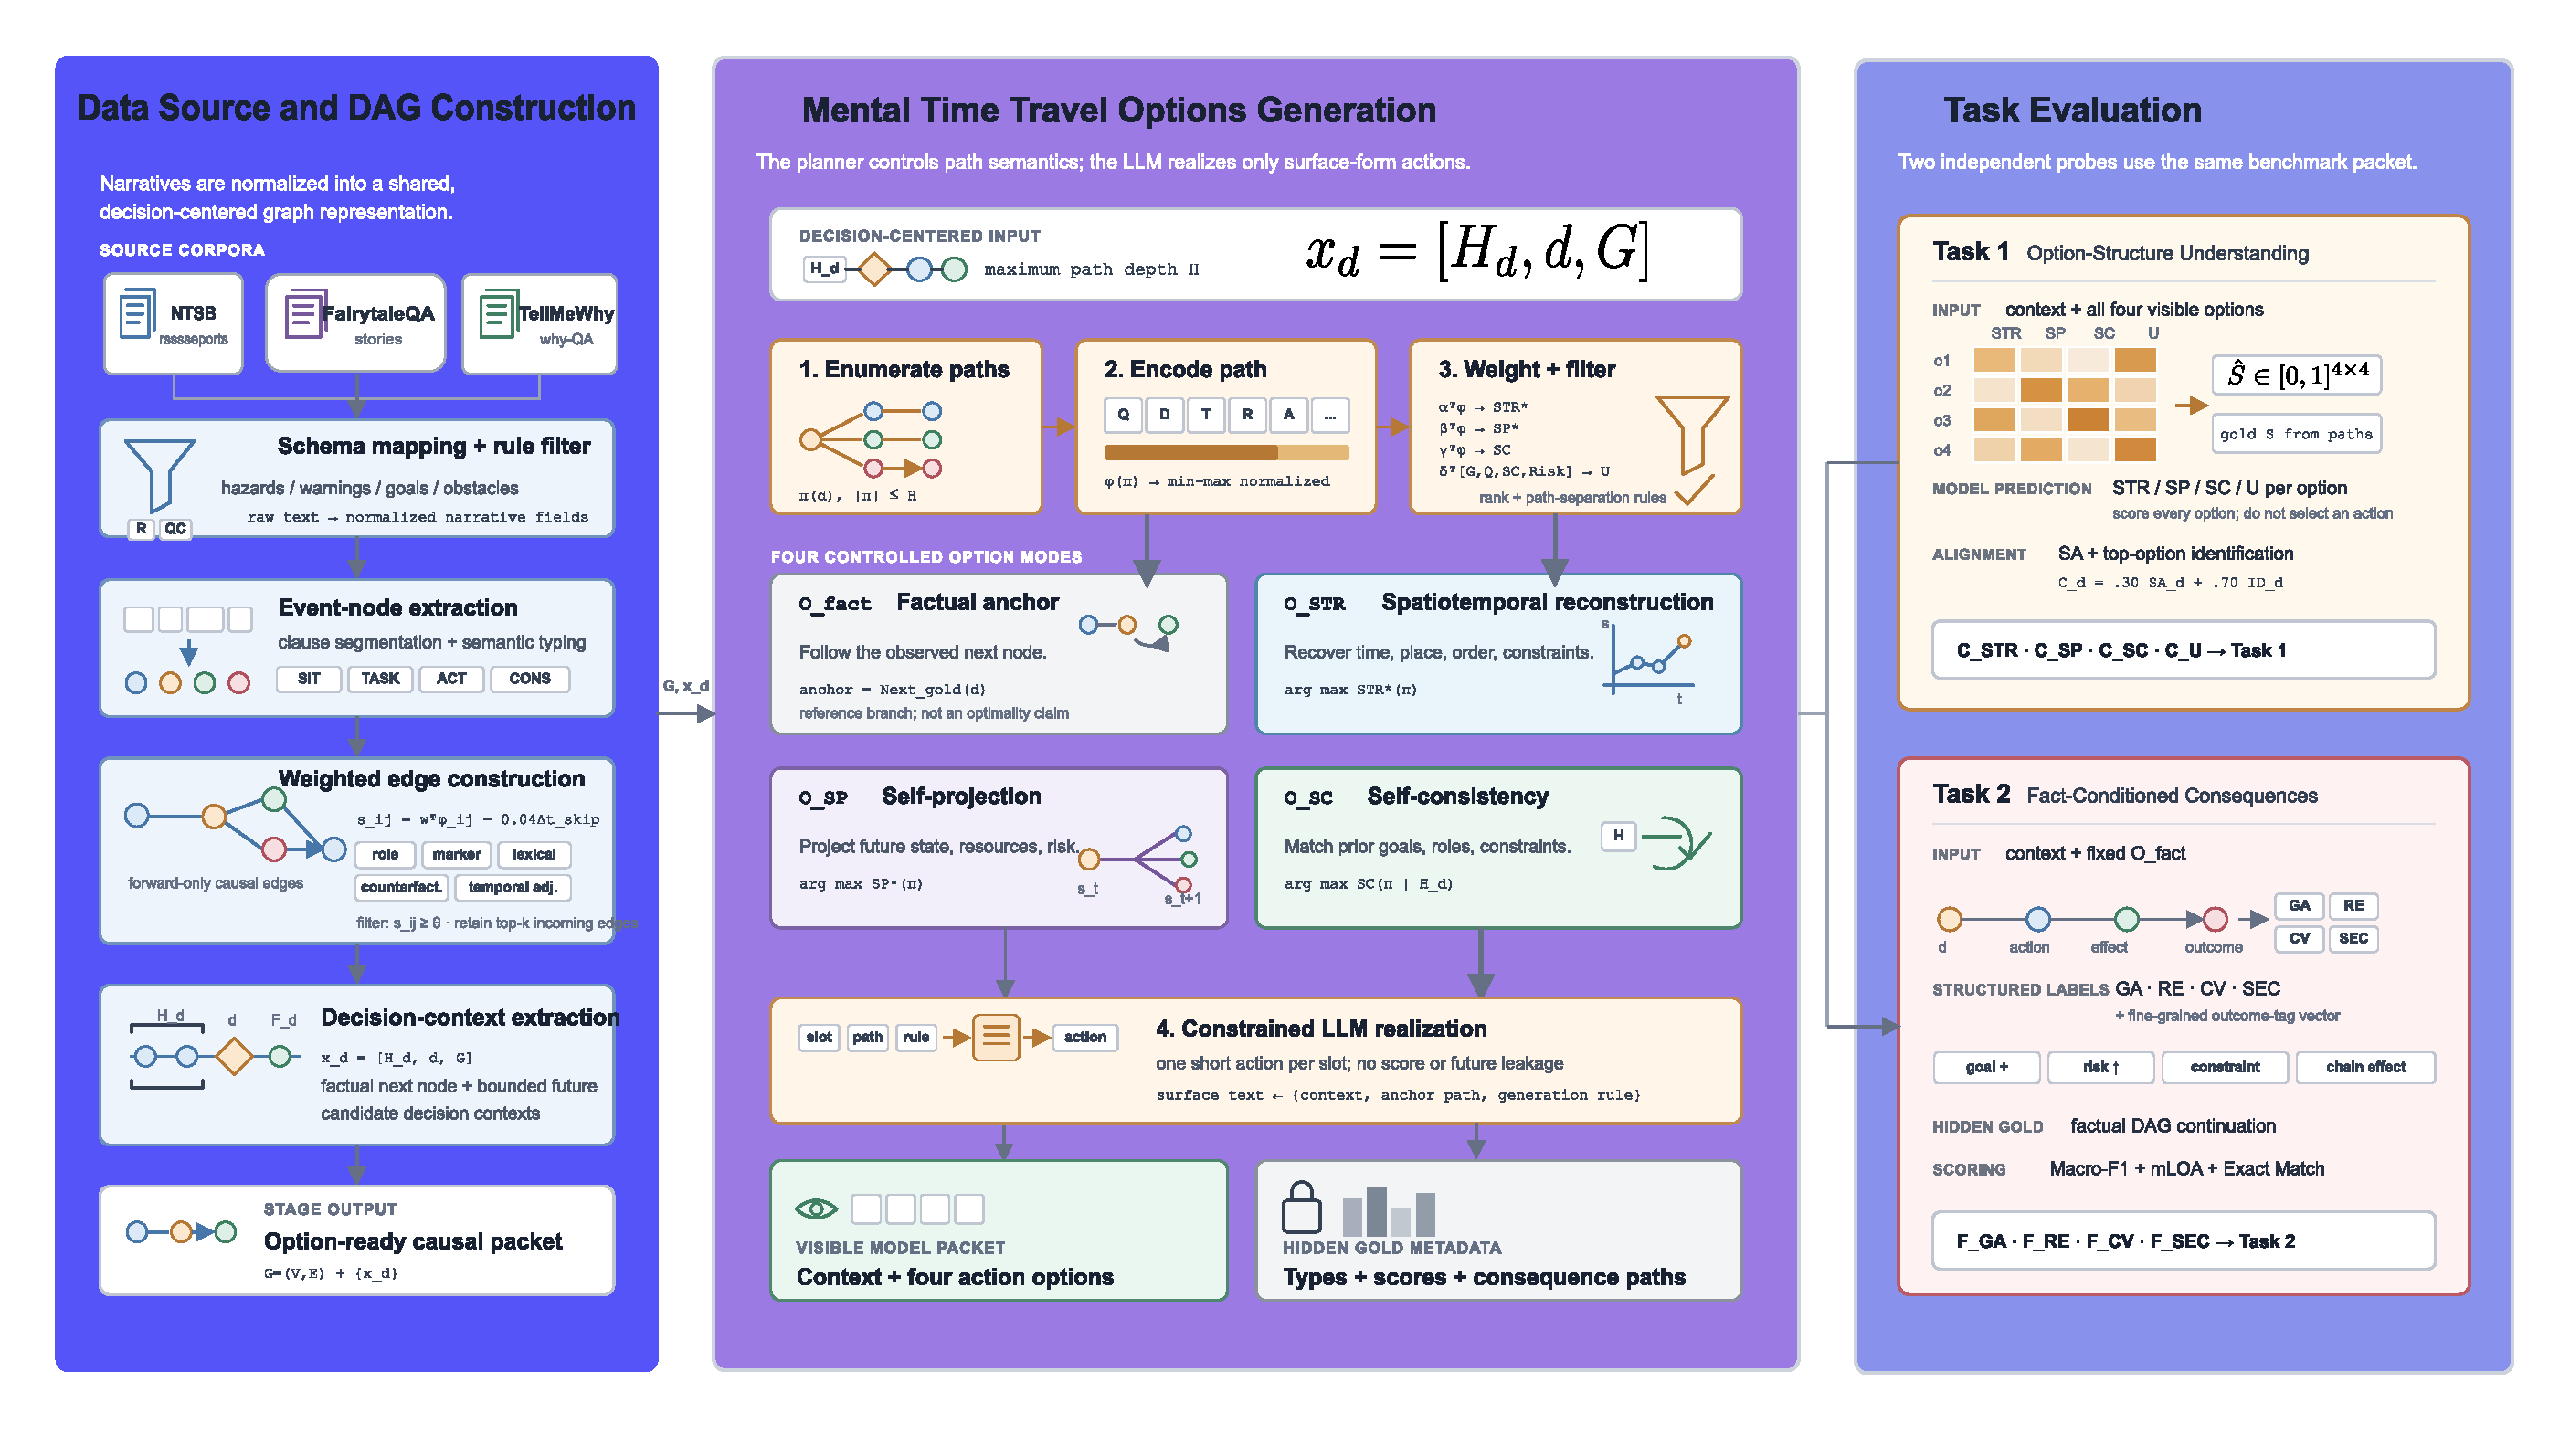
\includegraphics[width=1\linewidth]{mtt_algorithm_pipeline_figure.pdf}
\caption{Overview of the MTTravel-Bench construction and evaluation workflow.}
\label{fig:workflow}
\end{figure}
\paragraph{Narrative materials.}
This study draws on three publicly available narrative sources, including TellMeWhy, NTSB aviation accident investigation records, and FairytaleQA. These sources were selected not only to provide domain diversity, but also because they support the construction of decision-centered narrative trajectories. A usable sample in our benchmark must contain a recoverable prior state, one or more decision nodes, plausible action alternatives, and observable consequences that can be mapped into a DAG-based evaluation instance.

The three sources differ in narrative form and therefore contribute complementary reasoning structures. TellMeWhy provides short everyday narratives with more than 30,000 why-questions and free-form answers about why characters perform particular actions \cite{lal2021tellmewhy}. This source is useful for constructing low-risk commonsense decision cases, where actions are usually explained by ordinary goals, motivations, local constraints, and immediate consequences. NTSB aviation accident investigation records provide high-stakes risk narratives from public aviation investigation data \cite{ntsbCarol}. These cases often describe abnormal states, operational constraints, human responses, and delayed consequences under safety-critical conditions, making them suitable for testing risk anticipation and constraint-sensitive consequence prediction. FairytaleQA contains 278 children-friendly stories and 10,580 explicit and implicit QA pairs for narrative comprehension \cite{xu2022fantastic}. Compared with the other two sources, FairytaleQA is already a finely processed narrative dataset. Its stories usually contain coherent plots, rules, prohibitions, social relations, rescue arcs, and long-distance dependencies. For this reason, we use FairytaleQA as a reference form for narrative decomposition, and then screen NTSB and TellMeWhy cases that can be transformed into a similar decision-centered structure.

The filtering process follows three criteria. We first retain cases with moderate narrative length, because very short samples often lack sufficient prior state or consequence information, whereas overly long or highly technical samples are difficult to decompose into stable local decision nodes. We then require each retained case to contain a clear actor-action structure, an identifiable decision point, and a subsequent continuation that can support factual consequence labeling. Purely descriptive passages, duplicated cases, and samples without recoverable action-consequence structure are excluded. Finally, we balance the resulting benchmark primarily by the number of decision nodes rather than by the number of retained cases. This choice reflects the different narrative granularity of the three sources. FairytaleQA stories generally yield more decision nodes per case, TellMeWhy samples are shorter and yield fewer nodes, and NTSB cases fall between these two patterns. Balancing at the decision-node level allows each domain to contribute a comparable amount of evaluable reasoning structure.

After filtering, each retained narrative is processed into decision-centered units. The current balanced-suite configuration contains three narrative domains: 433 completed NTSB cases with 1,513 decision nodes, 232 FairytaleQA stories capped at 1,598 decision nodes, and 657 TellMeWhy narratives with 1,598 decision nodes. The evaluation unit is the decision-node prompt pair. Option generation and scoring are separated: a rule-guided construction model is used where graph repair or option verbalization is required, whereas model evaluation is performed by the fixed Task 1 and Task 2 scoring modules.

\begin{sidewaystable}[htbp]
\centering
\small
\caption{Data-source scale and benchmark roles}
\label{tab:data-source-scale-and-benchmark-roles}
\begin{tabular}{p{0.10\textwidth}p{0.10\textwidth}p{0.16\textwidth}p{0.20\textwidth}p{0.08\textwidth}p{0.05\textwidth}p{0.05\textwidth}p{0.16\textwidth}}
\toprule
Domain & Source & Original depicted & Filtering focus & Retained cases & Decision nodes & Nodes / case & Benchmark role \\
\midrule
High-stakes risk & NTSB completed aviation cases & Public aviation investigation records; CAROL aviation data available from 1962 to present & Recent completed cases with moderate length, clear anomaly-response-outcome chains, and observable consequences & 433 & 1,513 & 3.49 & Tests risk anticipation, constraint sensitivity, and delayed consequence prediction \\
Fictional long-horizon narrative & FairytaleQA & 278 stories; 10,580 QA pairs & Finely processed stories with coherent plots, rules, social relations, and long-distance dependencies & 232 & 1,598 & 6.89 & Tests long-range context use, rule-based inference, and abstract narrative consequence prediction \\
Everyday commonsense action & TellMeWhy & 30k+ why-questions and free-form answers over short narratives & Short everyday cases with clear actor motivation, local constraints, and ordinary action consequences & 657 & 1,598 & 2.43 & Tests goal inference, local constraint use, and ordinary consequence prediction \\
Total & -- & -- & -- & 1,322 & 4,709 & 3.56 &  \\
\bottomrule
\end{tabular}
\end{sidewaystable}

\paragraph{Context-to-DAG transformation.}
After source filtering, each retained case is converted into a causal-temporal DAG. The raw story, accident report, or QA item is not used directly as a benchmark instance. Each case is first transformed into a structured narrative trace that records the factual sequence of events, states, actions, constraints, and consequences in the source material. This transformation allows the benchmark to represent each case as a decision-centered structure, rather than as an unconstrained natural-language continuation task.

Let $\mathcal{E}=\{e_i\}_{i=1}^{N}$ denote the retained narrative case set. For each case $e_i$, the construction procedure builds an ordered event-clause trajectory rather than assuming that the narrative strictly alternates between states and actions. The source text is first segmented into sentences and clauses. A clause is retained when it contains cues related to state change, action, constraint, failure, goal, or outcome. Purely static background clauses are filtered out unless they express constraints that affect later action feasibility or consequence interpretation. The retained clauses form the factual backbone from which node order, factual successors, and decision contexts are derived.

\begin{equation}
\mathcal{E}=\{e_i\}_{i=1}^{N},\qquad
C_i=(c_{i,0},c_{i,1},\ldots,c_{i,T_i}).
\end{equation}


\begin{equation}
\tau_i^{*}=(v_{i,0},v_{i,1},\ldots,v_{i,T_i}),\qquad
\sigma_i(v_{i,t})=v_{i,t+1}.
\end{equation}

Each retained unit is normalized into a node $v_{i,t}$. The node stores its time index, source span, extracted subject, predicate, object or complement, optional result phrase, role, and semantic tags:
\begin{equation}
v_{i,t}=\langle \mathrm{id},t,\mathrm{span},\mathrm{subj},\mathrm{pred},\mathrm{obj},\mathrm{result},\mathrm{role},\mathrm{tags}\rangle .
\end{equation}
The role is assigned from the finite set $\{\mathrm{Situation},\mathrm{Task},\mathrm{Action},\mathrm{Consequence}\}$. The semantic tags further indicate cues such as goal, constraint, risk, failure, and outcome. Candidate decision nodes are then inferred from this normalized graph. A node is selected when it has a factual successor and its role is Task or Action. A Consequence node may also be selected when its factual successor is a Task or Action node. If no node satisfies these conditions, the procedure falls back to non-final nodes that have factual successors. In this way, decision-node selection is implemented as a role- and successor-constrained graph operation, rather than as a manual filter over pre-specified factual actions.

The construction process builds the graph directly from the extracted nodes using a set of explicit rules. For each pair of nodes $(v_{i,p}, v_{i,q})$, an edge is considered only when $p < q$ and $q-p \leq h$, where $h$ is the maximum allowed distance between nodes and is set to 5 by default. Each candidate edge is assigned a causal confidence score $w(e_{p,q})$, computed from role compatibility, explicit causal or temporal markers, lexical continuity, counterfactual plausibility, temporal adjacency, and a distance penalty:

\begin{equation}
w(e_{p,q})=0.30R_{p,q}+0.20M_{p,q}+0.20L_{p,q}+0.20C_{p,q}+0.10A_{p,q}-P_{p,q}.
\end{equation}
Here $R_{p,q}$ denotes role-pair compatibility, $M_{p,q}$ explicit causal or temporal markers, $L_{p,q}$ lexical continuity, $C_{p,q}$ counterfactual plausibility, $A_{p,q}$ temporal adjacency, and $P_{p,q}$ the distance penalty. An edge is kept if its score is at least $\theta = 0.25$. To control graph density, each node keeps at most $K = 3$ incoming edges with the highest scores. Because all edges point from earlier nodes to later nodes, the resulting graph is acyclic. Temporal adjacency contributes to the score but is not sufficient on its own to establish a causal relation.

\begin{equation}
e_{p,q}=(v_{i,p},v_{i,q}),\qquad p<q,\qquad q-p\le h,
\end{equation}
\begin{equation}
E_i=\operatorname{TopK}_{\mathrm{in}}\left(\{e_{p,q}\mid w(e_{p,q})\ge \theta\},K\right),\qquad \theta=0.25,\quad K=3,
\end{equation}
where $\operatorname{TopK}_{\mathrm{in}}$ keeps the strongest incoming edges for each target node.

In addition to this rule-based construction, the LLM takes the initial graph as input and modifies node boundaries, subject--predicate--object extraction, role and tag assignments, and weak or missing causal edges, while keeping consistency with the source text and temporal order. After this step, the graph is checked to ensure that node identifiers are valid, node text is non-empty, roles are legal, edges refer to existing nodes, all edges follow forward order, duplicates are removed, and scores fall within valid ranges. If the modified graph does not meet these conditions, the system reuses the original nodes or recomputes edges using the same scoring rules. Finally, the system updates the factual node order, successor relations, final node, decision nodes, and decision contexts. The overall construction therefore combines rule-based extraction, edge scoring, optional adjustment, and structural checking.

\begin{sidewaystable}[htbp]
\centering
\small
\caption{Rule schema for source-grounded DAG construction}
\label{tab:rule-schema-for-source-grounded-dag-cons}
\begin{tabular}{p{0.20\textwidth}p{0.35\textwidth}p{0.45\textwidth}}
\toprule
Construction step & Rule used in construction & Formal object in DAG \\
\midrule
Sentence and clause segmentation & The source text is segmented into ordered sentences and clauses. Clauses are retained when they contain state-change, action, constraint, failure, goal, or outcome cues, while pure background clauses are removed unless they express constraints. & Retained clause sequence $C_i = (c_{i,0}, c_{i,1}, \ldots, c_{i,T_i})$ \\
Event-node normalization & Each retained clause is converted into a graph node with extracted subject, predicate, object or complement, optional result phrase, role, and semantic tags. & Node $v_{i,t} = \langle span, subj, pred, obj, result, role, tags\rangle$ \\
Factual backbone construction & The retained node order is treated as the factual trajectory of the source narrative. Each non-final node receives a factual successor according to the observed order. & Factual trajectory $\tau_i^* = (v_{i,0}, v_{i,1}, \ldots, v_{i,T_i})$ and successor function $\sigma_i(v_{i,t}) = v_{i,t+1}$ \\
Candidate causal-edge scoring & Candidate edges are considered only for forward node pairs within the maximum skip window. Each pair is scored by role compatibility, explicit markers, lexical continuity, counterfactual plausibility, temporal adjacency, and distance penalty. & Candidate edge $e_{p,q}=(v_{i,p},v_{i,q})$, where $p<q$ and $q-p \leq h$, with confidence score $w(e_{p,q})$ \\
Edge thresholding and pruning & Edges are retained when their confidence score reaches the threshold. Dense targets are pruned by keeping only the strongest incoming edges. & Edge set $E_i = \operatorname{TopK}_{\mathrm{in}}(\{e_{p,q} \mid w(e_{p,q}) \geq \theta\},K)$, with at most $K$ incoming edges per target \\
Final-node inference & The final node is selected as the last Consequence node when one exists. Otherwise, the final factual node is used. & Final node $v_i^{final}$ \\
Decision-node inference & A node is retained as a decision node when it has a factual successor and its role is Task or Action. A Consequence node is also allowed when its successor is Task or Action. If no node satisfies these conditions, non-final nodes with factual successors are used as fallback candidates. & Decision-node set $D_i \subseteq V_i$ \\
LLM-assisted repair & The rule-generated baseline graph may be passed to an LLM for repairing node boundaries, extraction fields, roles, tags, and weak or missing source-grounded forward edges. The LLM does not generate answer options at this stage. & Repaired graph proposal $\tilde{G}_i=(\tilde{V}_i,\tilde{E}_i)$ \\
Local packaging and validation & The local validator checks node legality, forward-only edges, duplicate edges, score ranges, temporal order, and graph computability. Invalid proposals are corrected or replaced by the rule-based baseline. & Validated graph $G_i=(V_i,E_i)$, factual successor map $\sigma_i$, and decision contexts $H_d$ \\
\bottomrule
\end{tabular}
\end{sidewaystable}


\begin{equation}
D_i=\{d\in V_i\mid \sigma_i(d)\ \text{exists and}\ [\mathrm{role}(d)\in\{\mathrm{Task},\mathrm{Action}\}\ \text{or}\ 
(\mathrm{role}(d)=\mathrm{Consequence}\land \mathrm{role}(\sigma_i(d))\in\{\mathrm{Task},\mathrm{Action}\})]\},
\qquad
H_d=(v_{i,0},\ldots,d).
\end{equation}

The output of this stage is a source-grounded DAG $G_i=(V_i,E_i)$ for each retained case, together with factual successor maps, decision contexts, and a structurally validated decision-node set $D_i$. These outputs provide the structural basis for the next stage, where candidate future paths are enumerated and converted into factual and diagnostic action options.

\subsection{Option Generation and Mental-Time-Travel Alignment}
After the source-grounded DAG is constructed, each validated decision node is treated as a local option-generation site. For a retained case $e_i$, the previous stage provides a graph $G_i=(V_i,E_i)$, a factual successor function $\sigma_i$, a decision-node set $D_i$, and a decision context $H_d$ for each $d\in D_i$. Option generation is performed over this structured graph representation. The raw source text is no longer used as the direct generation input, so that every generated option can be traced to a node, path, or successor relation in the DAG.

For each decision node $d$, the planner enumerates bounded forward paths from $G_i$. A candidate path starts from $d$, follows directed edges in $E_i$, and preserves increasing temporal order. The maximum search depth is denoted by $L$, which is set to 3 in the benchmark construction. The candidate path set $\Pi_d$ is defined by the following constraint.

\begin{equation}
\Pi_d=\left\{\pi=(v_0,\ldots,v_\ell)\mid v_0=d,\ 1\le \ell\le L,\ \forall r\in\{1,\ldots,\ell\}:(v_{r-1},v_r)\in E_i,\ t(v_{r-1})<t(v_r)\right\}.
\end{equation}

The factual path is constructed from the factual successor function $\sigma_i$, rather than from the highest-scoring causal path. Starting from $d$, the factual path follows the observed successor relation in the source trajectory. When a factual successor transition is not included in the retained causal edge set $E_i$, the factual transition is still inserted into the candidate set as a source-grounded anchor. This design preserves the factual continuation even when the causal-edge pruning stage removes a local transition.

\begin{equation}
\pi_d^{\mathrm{fact}}=(d,\sigma_i(d),\sigma_i^2(d),\ldots,\sigma_i^{L}(d)).
\end{equation}

Each path $\pi\in\Pi_d$ receives a path quality score $Q(\pi)$. For paths composed of retained causal edges, $Q(\pi)$ is computed as the mean confidence score of the edges along the path. For factual-successor transitions inserted from $\sigma_i$ but absent from $E_i$, the transition score is set to $1.0$ in order to preserve the source-observed continuation. Thus, $Q(\pi)$ functions as a reliability term for option generation rather than as an independently estimated causal probability.

\begin{equation}
Q(\pi)=\frac{1}{|\pi|-1}\sum_{r=1}^{|\pi|-1} \bar{w}(v_{r-1},v_r),
\end{equation}
where $\bar{w}(u,v)=w(u,v)$ for retained causal edges and $\bar{w}(u,v)=1.0$ for source-observed factual-successor transitions inserted from $\sigma_i$.

The planner computes four families of path scores. The first three correspond to the functional MTT subcapacities used in this benchmark: spatiotemporal reconstruction (STR), self-projection (SP), and self-state or trajectory consistency (SC). STR measures whether an option requires reconstructing prior time, place, event order, causal setup, or constraints. SP measures whether an option requires projecting the future state of the acting subject, including ability, resources, opportunity, risk, or state change. SC measures whether an option remains consistent with the subject's prior role, goal, obligations, and local trajectory. The fourth score, $U$, is an auxiliary utility-oriented action-quality signal and is not treated as an MTT subcapacity.

These scores are derived from graph-level features rather than from surface option wording. The feature set includes path depth $D$, elapsed time-index distance $T$, role-transition ratio $R$, action-space change $A$, self-entity coverage $N_{self}$, self-action ratio $A_{self}$, self-state ratio $S_{self}$, tag continuity $K_{tag}$, role-pair continuity $K_{role}$, adjacent-time ratio $K_{time}$, final-node goal closeness $G$, and risk-tag ratio (Risk). The final-node goal closeness is defined using the distance from the path endpoint $v_m$ to the inferred final node $v_i^{final}$.

\begin{align}
D(\pi)&=|\pi|-1, &
T(\pi)&=t(v_m)-t(v_0),\\
R(\pi)&=\frac{1}{m}\sum_{r=1}^{m}\mathbb{1}[\mathrm{role}(v_r)\ne \mathrm{role}(v_{r-1})],&
A(\pi)&=1-\frac{|\mathcal{N}^+(v_0)\cap\mathcal{N}^+(v_m)|}{|\mathcal{N}^+(v_0)\cup\mathcal{N}^+(v_m)|+\epsilon}.
\end{align}

All scale-dependent features are normalized within the candidate path set of the same decision node. This local normalization prevents cross-domain variation in narrative length, graph density, and consequence granularity from dominating option selection. For a feature $x$, the normalized value is defined within $\Pi_d$. Features already bounded in $[0,1]$, including $Q,K_{tag},K_{role}$, and $K_{time}$, are used directly.

\begin{equation}
\widehat{x}(\pi)=
\frac{x(\pi)-\min_{\pi'\in\Pi_d}x(\pi')}
{\max_{\pi'\in\Pi_d}x(\pi')-\min_{\pi'\in\Pi_d}x(\pi')+\epsilon}.
\end{equation}

The score parameterization is fixed before model evaluation and is used consistently across all domains. The weights are determined through a construct-to-feature calibration protocol. This protocol first assigns each target construct to a compact set of graph features, then enforces local normalization, assigns larger weights to primary indicators of the construct, and checks whether selected option types remain stable under small perturbations of the weights. The resulting default configuration is denoted as $\Theta_0$. Alternative configurations are reserved for ablation and sensitivity analysis, while the main benchmark uses the fixed default parameterization.

\begin{equation}
\Theta_0=\{w_{\mathrm{STR}},w_{\mathrm{SP}},w_{\mathrm{SC}},w_U,L,\theta,\rho\}.
\end{equation}

\begin{sidewaystable}[htbp]
\centering
\small
\caption{Default parameterization for DAG-based option generation}
\label{tab:default-parameterization-for-dag-based-o}
\begin{tabular}{p{0.14\textwidth}p{0.18\textwidth}p{0.18\textwidth}p{0.14\textwidth}p{0.28\textwidth}}
\toprule
Score family & Construct measured & Feature group & Default weights & Rationale \\
\midrule
$\mathrm{STR}(\pi)$ & Spatiotemporal reconstruction & $\hat{D},\hat{T},\hat{R},\hat{A}$ & (0.30,0.30,0.20,0.20) & Path depth and elapsed narrative distance are primary indicators of reconstruction demand; role transition and neighborhood divergence provide structural separation. \\
$\mathrm{SP}(\pi)$ & Self-projection & $\hat{N}_{self},\hat{A}_{self},\hat{S}_{self}$ & (0.35,0.30,0.35) & Self-entity coverage and self-state change receive symmetric emphasis; self-action ratio captures whether the path remains actor-centered. \\
$\mathrm{SC}(\pi\mid H_d)$ & Self-state and trajectory consistency & $K_{tag},K_{role},K_{time},Q$ & (0.30,0.25,0.25,0.20) & Tag continuity is the strongest history-alignment signal; role continuity, temporal adjacency, and path quality provide additional consistency evidence. \\
$U(\pi)$ & Utility-oriented action quality & $G,Q,\mathrm{SC},Risk$ & (0.35,0.25,0.25,-0.15) & Goal closeness provides the main utility signal; path quality and consistency stabilize the estimate; risk contributes a negative penalty. \\
$\mathrm{STR}^{*}(\pi),\mathrm{SP}^{*}(\pi)$ & Reliability-weighted selection scores & $\mathrm{STR},\mathrm{SP},Q$ & Multiplicative $Q$ weighting & Reliability weighting prevents structurally attractive but weakly supported paths from dominating diagnostic option selection. \\
\bottomrule
\end{tabular}
\end{sidewaystable}

The resulting scoring functions are defined as follows. $\mathrm{STR}$, $\mathrm{SP}$, $\mathrm{SC}$, and $U$ are stored as the hidden option score profile; they define the diagnostic category of each option and support construction audit, but they are not treated as gold preference labels for model scoring. $\mathrm{STR}^{*}$ and $\mathrm{SP}^{*}$ are reliability-weighted selection scores used only to choose diagnostic option slots.

\begin{align}
\mathrm{STR}(\pi)&=0.30\widehat{D}+0.30\widehat{T}+0.20\widehat{R}+0.20\widehat{A},\\
\mathrm{SP}(\pi)&=0.35\widehat{N}_{\mathrm{self}}+0.30\widehat{A}_{\mathrm{self}}+0.35\widehat{S}_{\mathrm{self}},\\
\mathrm{SC}(\pi\mid H_d)&=0.30K_{\mathrm{tag}}+0.25K_{\mathrm{role}}+0.25K_{\mathrm{time}}+0.20Q(\pi),\\
U(\pi)&=0.35G(\pi)+0.25Q(\pi)+0.25\mathrm{SC}(\pi\mid H_d)-0.15\mathrm{Risk}(\pi),\\
\mathrm{STR}^{*}(\pi)&=\mathrm{STR}(\pi)Q(\pi),\qquad
\mathrm{SP}^{*}(\pi)=\mathrm{SP}(\pi)Q(\pi).
\end{align}

The option selector first constructs the factual option from $\pi_d^{\mathrm{fact}}$. It then selects diagnostic options by maximizing $\mathrm{STR}^{*}$, $\mathrm{SP}^{*}$, and $\mathrm{SC}$ under a separation constraint. The separation constraint removes exact duplicate paths, duplicate visible future nodes, and paths whose Jaccard similarity with already selected paths is at least $\rho$. The default threshold is $\rho=0.8$. If the strict constraint leaves no candidate for a diagnostic type, the selector falls back to the highest-scoring non-duplicate path with a distinct visible node. Let $\mathcal{C}_d(S)$ denote the candidate paths that remain after removing paths already in the selected set $S$, paths with duplicate visible nodes, and paths with $J(\pi,S)\ge \rho$.

\begin{align}
O_{\mathrm{fact}}&=\mathrm{Package}(\pi_d^{\mathrm{fact}}),\\
O_{\mathrm{STR}}&=\mathrm{Package}\!\left(\arg\max_{\pi\in\mathcal{C}_d(S)}\mathrm{STR}^{*}(\pi)\right),\\
O_{\mathrm{SP}}&=\mathrm{Package}\!\left(\arg\max_{\pi\in\mathcal{C}_d(S)}\mathrm{SP}^{*}(\pi)\right),\\
O_{\mathrm{SC}}&=\mathrm{Package}\!\left(\arg\max_{\pi\in\mathcal{C}_d(S)}\mathrm{SC}(\pi\mid H_d)\right).
\end{align}


\begin{equation}
O_d=\{O_{\mathrm{fact}},O_{\mathrm{STR}},O_{\mathrm{SP}},O_{\mathrm{SC}}\}
\quad\text{by default.}
\end{equation}

When enabled, an auxiliary utility option $O_{\mathrm{best}}$ is selected by maximizing $U(\pi)$ under the same separation constraint. This option is included as a rational-action reference and is not treated as a factual label or a gold answer.
In the LLM-backed generation mode, the same scoring functions are used to construct option slots. Each slot specifies the option type, factual flag, anchor path, target score profile, generation constraints, and visible-text constraints. The LLM is only used to verbalize non-factual actions under the slot constraints. The factual option is always packaged from the original factual successor node, and the generated visible text is not allowed to reveal hidden option types, scores, risk labels, or full future consequences.

The final selectable option set contains the factual option and up to three diagnostic counterfactual options by default. The utility option is included only when explicitly enabled. Each option has visible text and hidden metadata. The visible text contains a short first-step action, while the hidden metadata stores the anchor path, option type, score vector, hidden path, and consequence rubric.

\begin{equation}
M_{d,j}=\langle \pi_{d,j},\mathrm{type}_{d,j},z_{d,j},Y_{d,j},\mathrm{rubric}_{d,j}\rangle.
\end{equation}

The factual option has a stricter structured definition than the diagnostic counterfactual options. It is not the best action and is not a recommendation. It is the source-observed continuation anchored by the factual successor map. For each decision node, the hidden factual structure is

\begin{equation}
\Phi_d^{\mathrm{fact}}=\langle O_{\mathrm{fact}},\pi_d^{\mathrm{fact}},\Gamma_d^{\mathrm{fact}},y_d,Y_d\rangle ,
\end{equation}
where $\Gamma_d^{\mathrm{fact}}=(\sigma_i(d),\sigma_i^2(d),\ldots,\sigma_i^B(d))$ is the bounded factual consequence chain used in Task 2, with $B=4$ by default. The structured consequence vector is $y_d=(GA_d,RE_d,CV_d,SEC_d)$, where $GA$ denotes goal advancement, $RE$ risk evolution, $CV$ constraint violation, and $SEC$ secondary consequence. The local outcome tag set $Y_d\subseteq\mathcal{Y}$ records fine-grained consequences such as goal progress or failure, risk change, damage, loss of control, collision, landing outcome, constraint preservation or violation, resource change, injury, fire, weather exposure, and information gain. The tested model sees only the public context and visible action text; $\Phi_d^{\mathrm{fact}}$ is reserved for scoring.

\begin{sidewaystable}[htbp]
\centering
\small
\caption{Option types and their alignment with benchmark constructs}
\label{tab:option-types-and-constructs}
\begin{tabular}{p{0.20\textwidth}p{0.35\textwidth}p{0.35\textwidth}}
\toprule
Option & Graph source & Downstream role \\
\midrule
$O_{\mathrm{fact}}$ & Factual path derived from $\pi_d^{\mathrm{fact}}$ & Empirical anchor for fact-conditioned consequence prediction; not equivalent to optimality or recommendation. \\
$O_{\mathrm{STR}}$ & Separated path or slot anchor selected by $\mathrm{STR}^{*}$ & Tests spatiotemporal reconstruction: prior time, place, sequence, causal setup, and constraints. \\
$O_{\mathrm{SP}}$ & Separated path or slot anchor selected by $\mathrm{SP}^{*}$ & Tests self-projection: future subject state, resources, ability, opportunity, risk, and state change. \\
$O_{\mathrm{SC}}$ & Separated path or slot anchor selected by $\mathrm{SC}$ & Tests self-state and trajectory consistency: role, goal, obligation, constraint, and local history alignment. \\
$O_{\mathrm{best}}$ & Optional path or slot anchor selected by $U$ & Provides an auxiliary utility reference only when enabled; not generated by default and not treated as a gold answer. \\
\bottomrule
\end{tabular}
\end{sidewaystable}

The option-generation stage produces the hidden structures used by the two evaluation tasks. Task 1 records option-level model predictions over the visible options and derives a utility-implied preference profile over the option types. Task 2 fixes $O_{\mathrm{fact}}$ and uses the factual continuation to evaluate fact-conditioned consequence prediction. Algorithm~\ref{alg:dag-construction} summarizes the context-to-DAG transformation, and Algorithm~\ref{alg:option-generation} summarizes the option-generation procedure.

% Algorithms for MTTravel-Bench.

\begin{algorithm}\caption{Source-Grounded Narrative DAG Construction}
\label{alg:dag-construction}
\noindent\textbf{Input:} Source case $e_i$, segmentation rules, maximum skip window $h$, edge threshold $\theta$.\\
\textbf{Output:} Validated graph $G_i=(V_i,E_i)$, factual successor map $\sigma_i$, decision-node set $D_i$.
\begin{enumerate}
\item Segment the source text into ordered clauses $C_i=(c_{i,0},\ldots,c_{i,T_i})$.
\item Retain clauses that express state change, action, constraint, failure, goal, or outcome.
\item Normalize each retained clause into a node $v_{i,t}$ with span, subject, predicate, object, result, role, and tags.
\item Construct the factual trajectory $\tau_i^{*}=(v_{i,0},\ldots,v_{i,T_i})$ and successor map $\sigma_i(v_{i,t})=v_{i,t+1}$.
\item For each forward pair $(v_{i,p},v_{i,q})$ with $p<q$ and $q-p\le h$, compute confidence $w(e_{p,q})$ from role compatibility, markers, lexical continuity, counterfactual plausibility, temporal adjacency, and distance penalty.
\item Add $e_{p,q}$ to $E_i$ whenever $w(e_{p,q})\ge \theta$.
\item Keep at most $K$ highest-scoring incoming edges for each target node.
\item Infer the final node and decision-node set $D_i$ using role and successor constraints.
\item Optionally repair node boundaries, roles, tags, and weak edges with an LLM under source-grounded validation.
\item Validate node legality, forward-only edges, duplicate removal, score ranges, and graph computability.
\end{enumerate}
\end{algorithm}

\begin{algorithm}\caption{DAG-Based Option Generation}
\label{alg:option-generation}
\noindent\textbf{Input:} Validated graph $G_i$, decision node $d$, factual successor map $\sigma_i$, separation threshold $\rho$.\\
\textbf{Output:} Visible option set $O_d$ and hidden metadata $M_{d,j}$.
\begin{enumerate}
\item Enumerate bounded forward paths $\Pi_d$ from $d$ up to depth $L$.
\item Construct the factual path $\pi_d^{\mathrm{fact}}$ by following $\sigma_i$.
\item Insert factual-successor transitions into $\Pi_d$ when they were pruned from $E_i$.
\item For each $\pi\in\Pi_d$, compute $Q(\pi)$, normalized graph features, $\mathrm{STR}(\pi)$, $\mathrm{SP}(\pi)$, $\mathrm{STR}^{*}(\pi)$, $\mathrm{SP}^{*}(\pi)$, $\mathrm{SC}(\pi\mid H_d)$, and $U(\pi)$.
\item Set $S\gets \{O_{\mathrm{fact}}\}$, where $O_{\mathrm{fact}}=\mathrm{Package}(\pi_d^{\mathrm{fact}})$.
\item Select $O_{\mathrm{STR}}$, $O_{\mathrm{SP}}$, and $O_{\mathrm{SC}}$ by maximizing the corresponding score under duplicate and Jaccard-separation constraints.
\item If the utility option is enabled, select $O_{\mathrm{best}}$ by maximizing $U(\pi)$ under the same separation constraint.
\item For each $O_{d,j}\in O_d$, render visible first-step action text and store hidden metadata $M_{d,j}=\langle\pi_{d,j},\mathrm{type}_{d,j},z_{d,j},Y_{d,j},\mathrm{rubric}_{d,j}\rangle$, where $z_{d,j}=(\mathrm{STR},\mathrm{SP},\mathrm{SC},U)$ is the Task 1 target profile and the starred scores are retained as option-selection metadata.
\item Shuffle visible options before model evaluation.
\end{enumerate}
\end{algorithm}

\subsection{Tasks, Metrics, and Benchmark Reporting}
The benchmark evaluates models at key decision nodes in the source-grounded narrative DAG. For each evaluated decision node $(d\in\mathcal{D}_{\mathrm{eval}})$, the input consists of a decision context $H_d$ and a set of visible candidate actions $O_d=\{O_{d,1},\ldots,O_{d,K_d}\}$. The DAG provides the structural basis for locating the decision node, constructing candidate actions, assigning hidden structural profiles, and tracing factual continuations. The tested model observes only the decision context and the visible action texts. The hidden graph-derived metadata is used only for evaluation.

\paragraph{Task 1: utility-implied action preference profiling.}
Task 1 is defined as utility-implied action preference profiling at the same decision nodes. For model $m$ and decision node $d$, the response schema yields an option-level predicted profile for each visible candidate action, including a predicted utility $\widehat U_{m,d}(o)\in[0,1]$ for each option $o\in O_d$. The default option set $O_d=\{O_{\mathrm{fact}},O_{\mathrm{STR}},O_{\mathrm{SP}},O_{\mathrm{SC}}\}$ contains the factual continuation and three diagnostic options. $O_{\mathrm{fact}}$ packages the source-observed factual continuation and is neither an optimal action nor a recommendation. The three diagnostic options represent spatiotemporal reconstruction ($O_{\mathrm{STR}}$), self-projection ($O_{\mathrm{SP}}$), and self-state and trajectory consistency ($O_{\mathrm{SC}}$). These categories are defined by the graph-based option-construction procedure. They identify the analysis category of each option, but they are not gold preference labels.

A record is valid when its utility vector is finite and contains at least one positive value. Utilities are normalized within the decision node as
\begin{equation}
p_{m,d}(o)=\frac{\widehat U_{m,d}(o)}{\sum_{o'\in O_d}\widehat U_{m,d}(o')}.
\end{equation}
The utility-implied preferred option type is
\begin{equation}
\widetilde o_{m,d}=\arg\max_{o\in O_d}\widehat U_{m,d}(o),
\end{equation}
where the fixed benchmark option order is used only to resolve exact ties. Missing, non-finite, and uniformly zero utility vectors do not yield a preference proxy. Let $v_{m,d}\in\{0,1\}$ indicate whether a valid proxy is available. Preference coverage is
\begin{equation}
C_m=\frac{\sum_d v_{m,d}}{N_m},
\end{equation}
where $N_m$ is the number of synchronized Task 1 records for model $m$.

We report two complementary aggregates. The utility-implied selection share measures how often an option type receives the largest predicted utility,
\begin{equation}
\widehat P_m(o)=\frac{\sum_d\mathbb{1}[\widetilde o_{m,d}=o]v_{m,d}}{\sum_d v_{m,d}},
\end{equation}
whereas the mean probability mass retains the complete normalized utility distribution,
\begin{equation}
\overline p_m(o)=\frac{\sum_d p_{m,d}(o)v_{m,d}}{\sum_d v_{m,d}}.
\end{equation}
The dominant option type is $\arg\max_o\widehat P_m(o)$. Preference concentration is summarized using normalized entropy and the top-two utility margin,
\begin{align}
H_m&=\frac{1}{\sum_d v_{m,d}}\sum_d
\frac{-\sum_{o\in O_d}p_{m,d}(o)\log p_{m,d}(o)}{\log |O_d|}v_{m,d},\\
M_m&=\frac{1}{\sum_d v_{m,d}}\sum_d
\left(\widehat U_{m,d}^{(1)}-\widehat U_{m,d}^{(2)}\right)v_{m,d}.
\end{align}
Here, $\widehat U^{(1)}$ and $\widehat U^{(2)}$ are the largest and second-largest utilities. High $H_m$ or small $M_m$ indicates a diffuse rather than decisive profile. The Task 1 output is therefore
\begin{equation}
\mathrm{Task1Profile}_m=
\left(C_m,\{\widehat P_m(o)\}_o,\{\overline p_m(o)\}_o,H_m,M_m\right),
\end{equation}
not a scalar performance score or leaderboard.

Task 2 is defined as fact-conditioned consequence prediction at the same decision node. For each $d$, the factual action $O_{\mathrm{fact}}$, derived from the factual path $\pi_d^{\mathrm{fact}}$, is explicitly provided to the model together with $H_d$. The model is required to predict the consequence of following this factual action. Thus, Task 2 evaluates consequence prediction under a fixed action condition, rather than factual-action identification.

\begin{equation}
x_d=(H_d,O_{\mathrm{fact}}),\qquad O_{\mathrm{fact}}=\mathrm{Package}(\pi_d^{\mathrm{fact}}).
\end{equation}

The target for Task 2 contains two levels. The first level is a structured consequence vector $y_d$, which summarizes the global consequence profile of the factual continuation. It contains four dimensions. $GA_d$ denotes goal advancement and takes values in $\{\mathrm{none},\mathrm{partial},\mathrm{full}\}$. $RE_d$ denotes risk evolution and takes values in $\{\mathrm{decrease},\mathrm{neutral},\mathrm{increase}\}$. $CV_d$ denotes constraint violation and takes values in $\{\mathrm{no},\mathrm{yes}\}$. $SEC_d$ denotes the presence of secondary consequence and takes values in $\{\mathrm{no},\mathrm{yes}\}$.

\begin{equation}
y_d=(GA_d,RE_d,CV_d,SEC_d).
\end{equation}

The second level is a set of local outcome tags $Y_d$. These tags represent fine-grained state changes in the factual continuation and complement the structured consequence vector. The fixed tag vocabulary covers outcome categories such as goal completion, goal failure, risk change, damage, loss of control, collision, safe landing, rule violation, resource change, injury, fire, weather exposure, and information gain. The model output therefore contains both a structured prediction $\hat{y}_d$ and a tag-set prediction $\hat{Y}_d$.

The gold labels for Task 2 are derived from the factual continuation in the narrative DAG. Starting from the factual action, the evaluator follows the factual successor function $\sigma_i$ for a fixed consequence horizon $B$, where $B=4$ in the default setting. This produces a bounded continuation $\Gamma_d^{\mathrm{fact}}$. Node roles, semantic tags, and lexical cues in this continuation are mapped to $y_d$ and $Y_d$.

\begin{equation}
\Gamma_d^{\mathrm{fact}}=(\sigma_i(d),\sigma_i^2(d),\ldots,\sigma_i^{B}(d)),\qquad B=4.
\end{equation}

Task 2 scoring corresponds to this two-level target structure. At the structured-label level, the evaluator computes macro-F1 for each of the four consequence dimensions and averages them. At the local-outcome level, it computes micro-F1 between predicted and gold outcome tags. Exact match over the four-dimensional structured vector is included as a stricter consistency measure.

\begin{align}
\mathrm{LabelF1}&=\frac{1}{4}\sum_{k\in\{GA,RE,CV,SEC\}}\mathrm{MacroF1}_k,\\
P_{\mathrm{LOA}}&=\frac{\sum_{d\in\mathcal{D}_{\mathrm{eval}}} |\hat{Y}_d\cap Y_d|}{\sum_{d\in\mathcal{D}_{\mathrm{eval}}} |\hat{Y}_d|+\epsilon},\qquad
R_{\mathrm{LOA}}=\frac{\sum_{d\in\mathcal{D}_{\mathrm{eval}}} |\hat{Y}_d\cap Y_d|}{\sum_{d\in\mathcal{D}_{\mathrm{eval}}} |Y_d|+\epsilon},\\
\mathrm{mLOA}&=\frac{2P_{\mathrm{LOA}}R_{\mathrm{LOA}}}{P_{\mathrm{LOA}}+R_{\mathrm{LOA}}+\epsilon},\\
\mathrm{StructuredScore}&=0.90\,\mathrm{LabelF1}+0.10\,\mathrm{EM}.
\end{align}

The final Task 2 score assigns equal primary weight to the two evidence layers, because structured labels and local outcome tags capture complementary aspects of consequence prediction. The exact-match term is retained as a smaller consistency component.

\begin{equation}
\mathrm{Task2}=0.45\,\mathrm{LabelF1}+0.45\,\mathrm{mLOA}+0.10\,\mathrm{EM}.
\end{equation}

Score aggregation follows the hierarchical structure of the benchmark. The basic evaluation unit is the decision node, but final reporting is performed at the case and domain levels to account for variation in narrative length and decision-node density. For a case $e_i$, let $D_i$ denote its evaluated decision-node set and $S_d$ denote the score of decision node $d$. The case-level score is

\begin{equation}
S(e_i)=\frac{1}{|D_i|}\sum_{d\in D_i}S_d.
\end{equation}

For each source domain $g$, let $E_g$ denote the retained cases from that domain. The domain-level score and final macro-average are defined as

\begin{align}
S(g)&=\frac{1}{|E_g|}\sum_{e_i\in E_g}S(e_i),\\
S_{\mathrm{macro}}&=\frac{1}{|\mathcal{G}|}\sum_{g\in\mathcal{G}}S(g).
\end{align}

Task 1 and Task 2 are reported side by side but are not averaged. A larger Task 1 selection share indicates a more frequent utility-implied orientation toward one option type, not better performance. A larger Task 2 score indicates closer agreement with the factual continuation. Combining the two would impose an unsupported normative ordering on Task 1 and would yield a composite without a stable interpretation; accordingly, no cross-task composite score is computed. Reporting the Task 1 preference profile next to the Task 2 score and its components allows the benchmark to distinguish candidate-action orientation from fact-conditioned consequence prediction.

\begin{equation}
\mathrm{BaselineAdjusted}(S)=\frac{S-S_{\mathrm{baseline}}}{1-S_{\mathrm{baseline}}}.
\end{equation}
The baseline-adjusted score is used only as a deterministic non-human difficulty reference for Task 2 diagnostics, and negative values indicate performance below the deterministic baseline for that metric. The Task 1 preference profile and the raw Task 2 score with its component profile remain the primary reported measurements.

\paragraph{Evaluation protocol.}
The experimental protocol follows the implemented two-task evaluation pipeline rather than a free-form model-comparison setup. All evaluated models receive the same public decision context, the same visible candidate actions, and the same JSON output schemas generated by the benchmark runner. Task 1 uses option-level STR, SP, SC, and U score prediction, from which the utility-implied preference profile is derived. Task 2 fixes the factual option and evaluates structured consequence labels and fine-grained outcome tags. The hidden DAG metadata, target\_generation\_scores, factual successor chain, and outcome-tag targets are used only by the scoring program.

\paragraph{Synchronized panel and statistical analysis.}
The synchronized comparison panel contained 30 models evaluated with identical prompts, option order, response schemas, and scoring code. The current result tables contained 4,453 common evaluable decision nodes per model: 1,444 from NTSB, 1,466 from FairytaleQA, and 1,543 from TellMeWhy, all drawn from the balanced three-domain suite. This produced 133,590 model--node records for Task 1 preference extraction. All valid records contributed to descriptive profiles, while the primary cross-task analysis was restricted to models with $C_m\geq0.80$.

For each option type, domain differences in $\widehat P_m(o)$ were tested using a model-paired Friedman test, followed by paired Wilcoxon signed-rank contrasts with Benjamini--Hochberg correction over 12 comparisons. Task 2 domain differences were evaluated using one paired Friedman test and three corrected paired contrasts. The primary cross-task analysis computed Spearman correlations between Task 1 preference descriptors and Task 2 for the 26 models meeting the coverage threshold. The conservative prespecified 20-test correction family was retained, and all 30 models were included only as a coverage sensitivity analysis. The models were not rerun and no raw Task 1 or Task 2 outputs were altered.
\begin{table}[htbp]
\centering
\small
\caption{Model-panel design and evaluation rationale}
\label{tab:model-panel-design-and-evaluation-ration}
\begin{tabular}{p{0.20\textwidth}p{0.35\textwidth}p{0.35\textwidth}}
\toprule
Experimental axis & Implemented control & Rationale \\
\midrule
Dataset and scale & Balanced three-domain suite with decision-node-level accounting & Separates domain effects from the number of evaluable decision points. \\
Model family & Provider/model families are evaluated with identical prompts and output schemas & Tests whether the benchmark captures general narrative-reasoning ability rather than a provider-specific behavior. \\
Model size and cost tier & Compact, mid-tier, and larger/frontier models can be compared in the same runner & Assesses whether Task 1 profile recovery and Task 2 consequence prediction show capacity-sensitive patterns. \\
Reasoning mode & Reasoning and non-reasoning variants are kept as distinct model entries when available & Tests whether explicit reasoning improves factual consequence prediction or instead increases unsupported outcome generation. \\
Scoring and baselines & Frozen Task 1/Task 2 scoring plus deterministic baseline-only adjustment & Keeps construct scores primary while providing a non-human difficulty reference. \\
\bottomrule
\end{tabular}
\end{table}

The broad model panel is necessary because MTTravel-Bench is intended as a measurement instrument, not merely as a leaderboard. Evaluating only one frontier model would make it impossible to distinguish benchmark difficulty from the idiosyncrasies of a single provider, decoding stack, or instruction-following style. Therefore, the implemented configuration supports a large set of models that differ in family, scale, cost tier, context capacity, and reasoning mode, while holding prompts, data splits, task definitions, and scoring scripts fixed.

This design also addresses construct validity. Model size is expected to affect long-context state tracking and numerical profile calibration; model family may affect causal-temporal priors and domain robustness; reasoning-oriented variants may improve consequence prediction but may also overgenerate unsupported outcomes; compact models test whether the benchmark is sensitive to capacity limitations and JSON-schema compliance. Reporting Task 1, Task 2, their capability profiles, deterministic baseline-adjusted scores, and domain-stratified summaries makes these differences interpretable without relying on human-performance comparison.

Table~\ref{tab:worked-task-example} illustrates the complete measurement pipeline with one worked decision node per domain, covering option generation, Task 1 preference profiling, and Task 2 consequence prediction on the same source-grounded instances.

\begin{sidewaystable}[p]
\centering
\caption{Sequential examples of option generation, Task~1 preference profiling, and Task~2 consequence prediction across NTSB, FairytaleQA, and TellMeWhy.}
\label{tab:worked-task-example}
\footnotesize
\setlength{\tabcolsep}{3.5pt}
\renewcommand{\arraystretch}{1.10}
\begin{tabular}{p{0.19\textwidth}p{0.248\textwidth}p{0.248\textwidth}p{0.248\textwidth}}
\toprule
\textbf{Pipeline stage} &
\textbf{NTSB accident report} &
\textbf{FairytaleQA narrative} &
\textbf{TellMeWhy everyday event} \\
\midrule
\raggedright\textbf{Option Generation}\par
\textit{Input:} source-grounded decision context\par
\textit{Output:} four typed candidate actions
&
\textbf{Context.} During a touch-and-go landing, a wind gust lifts the tail. The airplane lands hard, loses its nose wheel, and stops nose-down with substantial damage.\par
\textbf{Generated actions.}\par
1. Report no preaccident malfunction \textit{(factual continuation)}.\par
2. Reconstruct the landing sequence \textit{(spatiotemporal reconstruction)}.\par
3. Secure the aircraft and occupants \textit{(self-projection)}.\par
4. Notify airport personnel \textit{(self-state and trajectory consistency)}.
&
\textbf{Context.} Korbes returns home after the animals and household objects have positioned themselves around the house.\par
\textbf{Generated actions.}\par
1. Go to the hearth and make a fire \textit{(factual continuation)}.\par
2. Check the barn \textit{(spatiotemporal reconstruction)}.\par
3. Light a lantern \textit{(self-projection)}.\par
4. Call through the house \textit{(self-state and trajectory consistency)}.
&
\textbf{Context.} Cam orders a pizza, takes it home, and opens the box to take out a slice.\par
\textbf{Generated actions.}\par
1. Discover that the pizza is uncut \textit{(factual continuation)}.\par
2. Call the pizza shop \textit{(spatiotemporal reconstruction)}.\par
3. Get a cutting board \textit{(self-projection)}.\par
4. Use a kitchen knife \textit{(self-state and trajectory consistency)}.
\\
\midrule
\raggedright\textbf{Task 1}\par
\textit{Utility-Implied Action Preference Profiling}\par
\textit{Input:} context and four generated actions\par
\textit{Output:} option-level STR/SP/SC/U profile and U-implied preference record
&
\textbf{Dominant labels.}\par
\textbf{SC:} Report no preaccident malfunction (0.90).\par
\textbf{STR:} Reconstruct the landing sequence (0.90).\par
\textbf{U: Secure the aircraft and occupants (0.90).}\par
\textbf{U:} Notify airport personnel (0.80).\par
\textbf{U-implied preference:} Secure the aircraft and occupants (U = 0.90; self-projection).\par
\textbf{Preference characteristic.} The highest utility is assigned to an intervention that changes the agent's immediate safety state.
&
\textbf{Dominant labels.}\par
\textbf{SC: Go to the hearth and make a fire (0.90).}\par
\textbf{SC:} Check the barn (0.60).\par
\textbf{SC:} Light a lantern (0.50).\par
\textbf{SC:} Call through the house (0.40).\par
\textbf{U-implied preference:} Go to the hearth and make a fire (U = 0.80; factual continuation).\par
\textbf{Preference characteristic.} The highest utility is assigned to continuing the source narrative rather than introducing an alternative branch.
&
\textbf{Dominant labels.}\par
\textbf{STR:} Discover that the pizza is uncut (0.80).\par
\textbf{SP:} Call the pizza shop (0.60).\par
\textbf{SP:} Get a cutting board (0.80).\par
\textbf{U: Use a kitchen knife (0.90).}\par
\textbf{U-implied preference:} Use a kitchen knife (U = 0.90; self-state and trajectory consistency).\par
\textbf{Preference characteristic.} The highest utility is assigned to an action that preserves continuity between Cam's current goal and the next step.
\\
\midrule
\raggedright\textbf{Task 2}\par
\textit{Fact-Conditioned Consequence Prediction}\par
\textit{Input:} context and fixed factual action\par
\textit{Output:} consequence relation, structured labels, and local outcomes
&
\textbf{Fixed factual action.} Report that no preaccident mechanical malfunction prevented normal operation.\par
\textbf{Consequence relation.} The report rules out a mechanical-failure explanation, while the hard landing and resulting damage remain in the predicted outcome.\par
\textbf{Structured labels.} Goal status: none; risk effect: neutral; constraint violation: no; secondary consequence: no.\par
\textbf{Local outcomes.} Goal failure, damage, hard landing, and information gain.
&
\textbf{Fixed factual action.} Korbes goes to the hearth to make a fire.\par
\textbf{Consequence relation.} Approaching the hearth triggers the hidden objects, increasing danger and leading to injury.\par
\textbf{Structured labels.} Goal status: none; risk effect: increase; constraint violation: no; secondary consequence: yes.\par
\textbf{Local outcomes.} Increased risk, fire, secondary consequence, and injury.
&
\textbf{Fixed factual action.} Cam discovers that the store did not cut the pizza.\par
\textbf{Consequence relation.} The uncut pizza blocks immediate eating and adds a handling step, which the output treats as partial progress, increased risk, and a secondary consequence.\par
\textbf{Structured labels.} Goal status: partial; risk effect: increase; constraint violation: no; secondary consequence: yes.\par
\textbf{Local outcomes.} Partial goal progress, increased risk, information gain, and a secondary consequence.
\\
\bottomrule
\end{tabular}
\end{sidewaystable}

\section{Results}
\label{sec:mttravel-results}

\subsection{Evaluation Coverage}

The synchronized analysis compared 30 models on 4,453 common evaluable decision nodes per model, drawn from the balanced 1,322-case suite described in Section~\ref{sec3}. Task~1 yielded 125,623 valid utility-implied preference records from 133,590 model--node records, corresponding to 94.0\% aggregate coverage. Twenty-six models had $C_m\geq0.80$ and formed the primary Task~1--Task~2 association cohort; the remaining four models were retained only for sensitivity visualization and the all-model sensitivity test. This separation prevented incomplete utility outputs from being interpreted as substantive preferences.

\subsection{Task 1 Preference Structure and Cross-Task Association}

Task~1 produced heterogeneous selection-share profiles rather than a scalar winner. Self-projection was the most frequent dominant option type, but the model profiles varied substantially and shifted across domains. Figure~\ref{fig:task1-preference-structure} connects the three parts of the evidence: panel~a establishes model-level heterogeneity, panel~b tests domain conditioning, and panel~c evaluates the only preference descriptor that retained a corrected association with Task~2.

\begin{figure}[p]
\centering
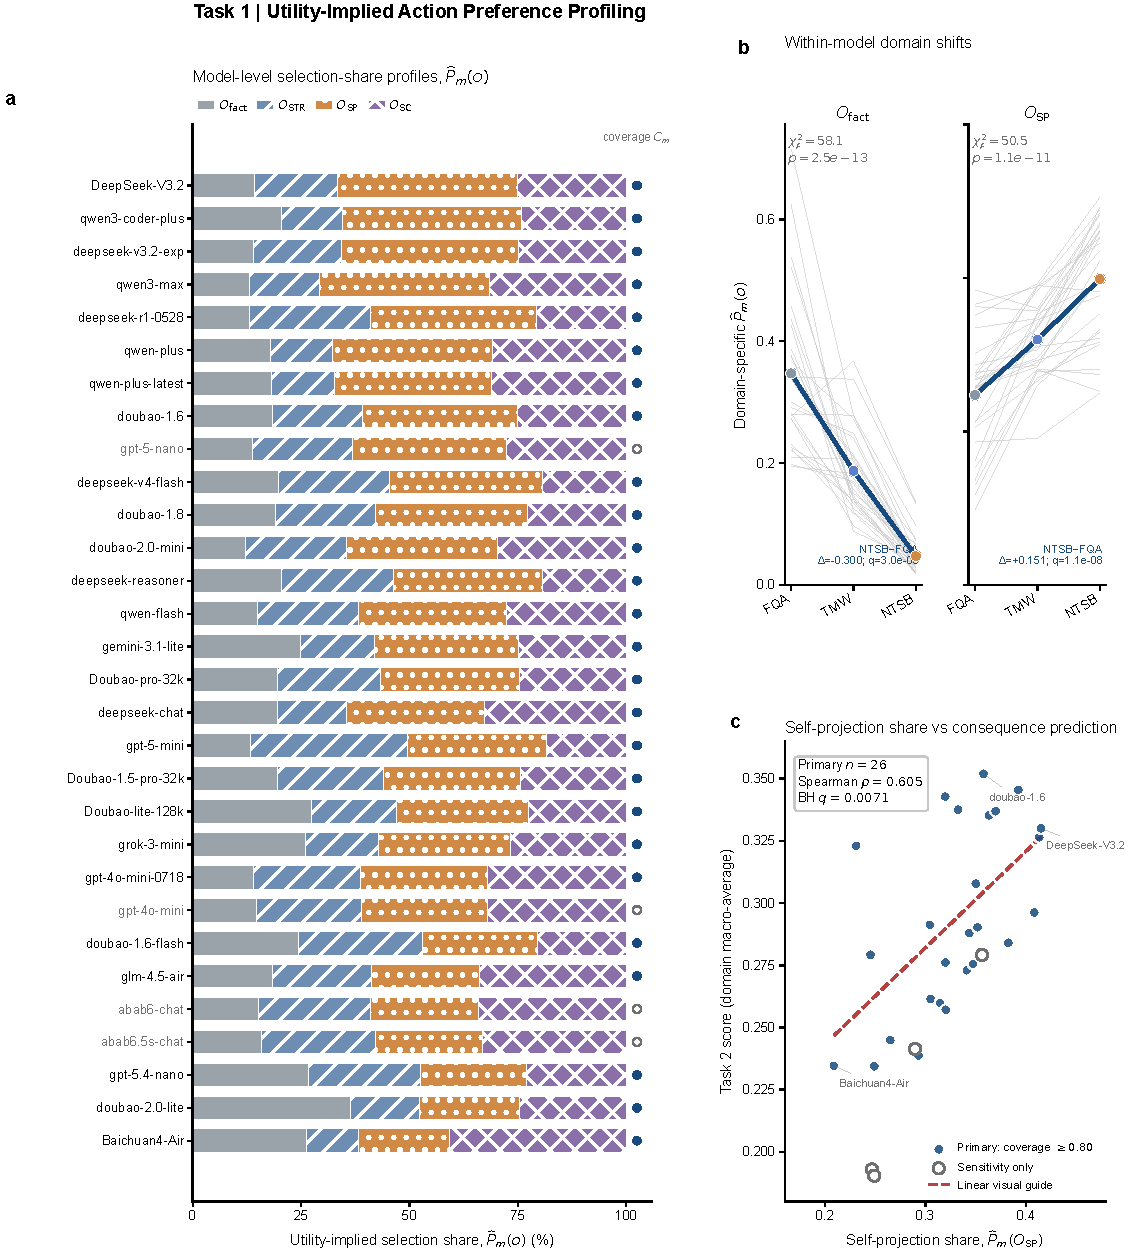
\includegraphics[width=0.96\textwidth]{figure_1_preference_structure_and_task2_association.pdf}
\caption{\textbf{Utility-implied preference structure and its selective association with fact-conditioned consequence prediction.} \textbf{a}, Utility-implied selection-share profiles $\widehat P_m(o)$ for 30 synchronized models. Across 125,623 valid records, the instance-weighted shares were 32.59\% for self-projection ($O_{\mathrm{SP}}$), 26.65\% for self-state and trajectory consistency ($O_{\mathrm{SC}}$), 21.51\% for spatiotemporal reconstruction ($O_{\mathrm{STR}}$), and 19.25\% for the source-observed factual continuation ($O_{\mathrm{fact}}$). Nineteen models were $O_{\mathrm{SP}}$-dominant, seven were $O_{\mathrm{SC}}$-dominant, two were $O_{\mathrm{STR}}$-dominant, and two were $O_{\mathrm{fact}}$-dominant. Filled markers indicate the primary coverage cohort ($C_m\geq0.80$); open markers indicate sensitivity-only models. \textbf{b}, Model-paired domain trajectories for the two strongest contrasts. From FairytaleQA to NTSB, the valid-record-weighted $O_{\mathrm{fact}}$ share decreased from 34.44\% to 4.74\%, whereas the $O_{\mathrm{SP}}$ share increased from 25.32\% to 40.08\%. Friedman tests detected domain effects for $O_{\mathrm{fact}}$ ($\chi_F^2=58.07$, $p=2.46\times10^{-13}$) and $O_{\mathrm{SP}}$ ($\chi_F^2=50.47$, $p=1.10\times10^{-11}$); the NTSB--FairytaleQA model-mean contrasts were $-0.300$ ($q=2.97\times10^{-6}$) and $+0.151$ ($q=1.12\times10^{-8}$), respectively. Grey lines denote individual models and coloured points denote domain means ($n=30$ paired models). \textbf{c}, Association between self-projection selection share $\widehat P_m(O_{\mathrm{SP}})$ and Task~2. In the primary cohort ($n=26$), Spearman $\rho=0.605$, $p=0.0011$, and BH-adjusted $q=0.0071$; the dashed least-squares line is a visual guide rather than the inferential model. Together, panels a--c show that the Task~1 proxy is heterogeneous and domain-conditioned, with one selective model-level link to Task~2. They do not establish explicit action choice or causality. Source data are provided with the figure package.}
\label{fig:task1-preference-structure}
\end{figure}

\subsection{Task 2 Performance Profile}

Task~2 separated models, diagnostic components, and narrative domains. The overall ranking contained a relatively close leading group, while the component and domain leaders differed. Figure~\ref{fig:task2-performance-profile} therefore treats the Task~2 score as a profile with three diagnostic views rather than as sufficient evidence for a single universally best model.

\begin{figure}[p]
\centering
    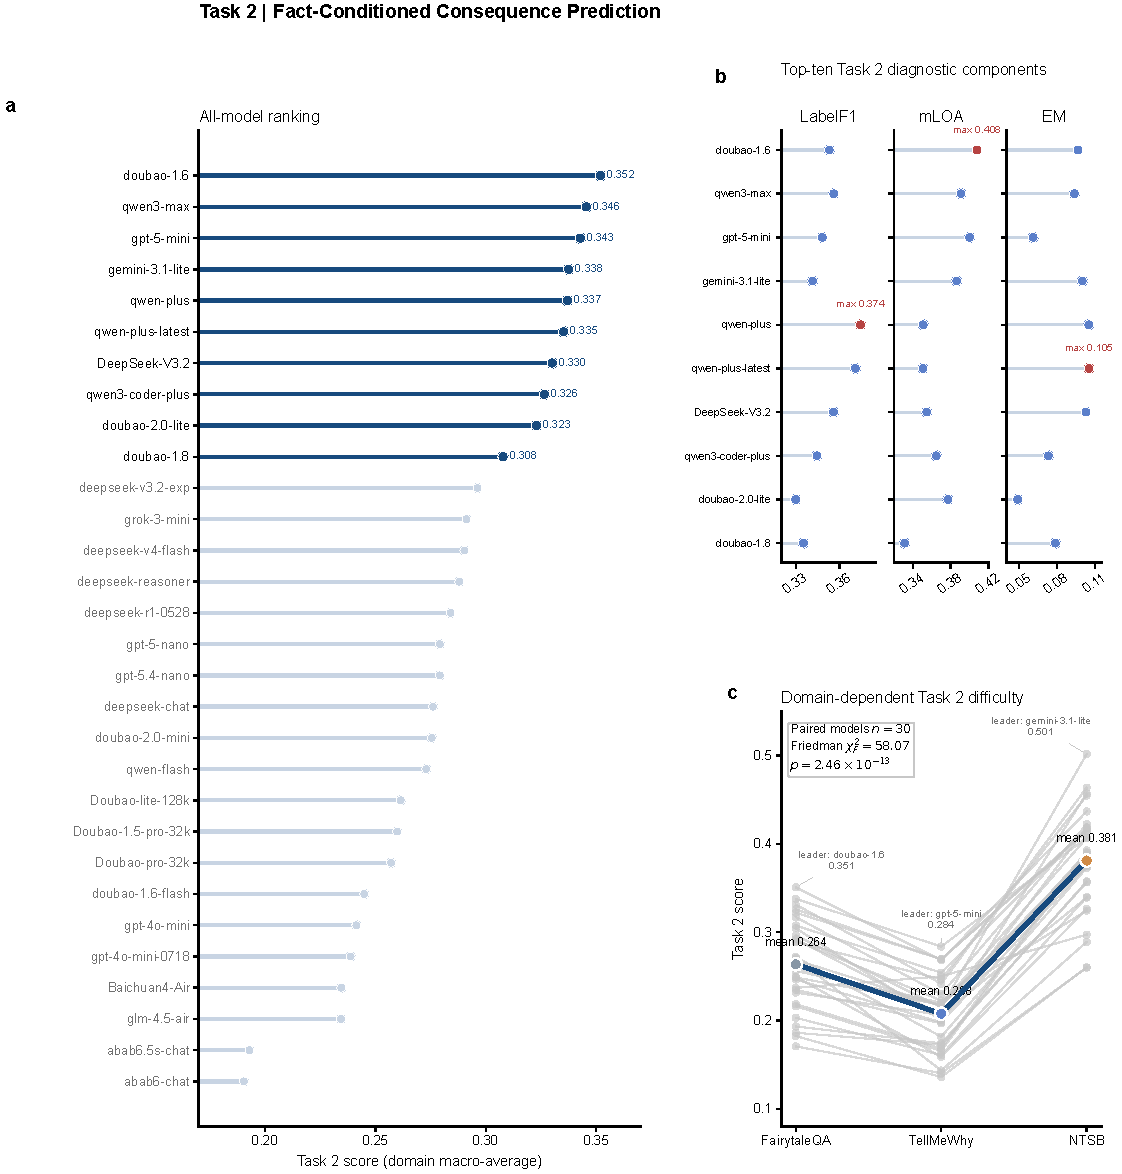
\includegraphics[width=1\linewidth]{figure_2_task2_performance_decomposition.pdf}
\caption{\textbf{Fact-conditioned consequence prediction varies across models, diagnostic components, and narrative domains.} \textbf{a}, Task~2 scores for all 30 models, aggregated within case and domain and then macro-averaged across the three domains. The four highest scores were 0.352, 0.346, 0.343, and 0.338, leaving a first-to-fourth gap of 0.014; the ten highest-scoring models are highlighted. \textbf{b}, Raw LabelF1, mLOA, and EM values for the top ten models. The component maxima were 0.374 for LabelF1, 0.408 for mLOA, and 0.105 for EM, and were achieved by different models. LabelF1 averages macro-F1 over goal advancement, risk evolution, constraint violation, and secondary consequence; mLOA is micro-F1 over local outcome-tag sets; EM is exact match over the complete structured consequence vector. Red points denote the maximum within each displayed component. \textbf{c}, Model-paired domain Task~2 scores. The 30-model means were 0.264 for FairytaleQA, 0.208 for TellMeWhy, and 0.381 for NTSB; different models led the three domains at 0.351, 0.284, and 0.501, respectively. A paired Friedman test detected a domain effect ($\chi_F^2=58.07$, $p=2.46\times10^{-13}$). Grey lines denote individual models and coloured points denote domain means ($n=30$ paired models). Together, the panels show that Task~2 does not reduce to a stable one-dimensional capability: overall rank, component strength, and domain leadership provide non-equivalent information. Source data are provided with the figure package.}
\label{fig:task2-performance-profile}
\end{figure}

\FloatBarrier

\section{Experimental Analysis}
\label{sec:mttravel-analysis}

\subsection{Task 1 Profiles Are Heterogeneous but Graded}

\paragraph{Preference profiling does not define a Task 1 leaderboard.}
The 30-model panel contained 19 $O_{\mathrm{SP}}$-dominant models, seven $O_{\mathrm{SC}}$-dominant models, two $O_{\mathrm{STR}}$-dominant models, and two $O_{\mathrm{fact}}$-dominant models. The valid-record-weighted selection shares followed the same ordering: 0.326 for $O_{\mathrm{SP}}$, 0.267 for $O_{\mathrm{SC}}$, 0.215 for $O_{\mathrm{STR}}$, and 0.193 for $O_{\mathrm{fact}}$ (Fig.~\ref{fig:task1-preference-structure}a and Table~\ref{tab:preference_profiles}). These values establish a predominantly self-projection-oriented aggregate pattern, but they do not define an accuracy ranking because no option type is a normative gold preference.

\paragraph{Dominance did not imply sharp separation.}
The model-mean probability masses were 0.177, 0.261, 0.286, and 0.277 for $O_{\mathrm{fact}}$, $O_{\mathrm{STR}}$, $O_{\mathrm{SP}}$, and $O_{\mathrm{SC}}$, respectively. Mean normalized entropy was 0.907 and the mean top-two utility margin was 0.135. Thus, the highest-utility option often held only a limited advantage over alternatives. The Task~1 evidence supports graded preference geometry, not four sharply separated classes of models.

\begin{table}[p]
\centering
\caption{Task~1 utility-implied action preference profiles overall and by domain. Values are valid-record-weighted selection shares $\widehat P_m(o)$ (\%).}
\label{tab:preference_profiles}
\small
\setlength{\tabcolsep}{5.0pt}
\begin{tabular}{lrrrrrr}
\toprule
Scope & Valid/total records & $O_{\mathrm{fact}}$ & $O_{\mathrm{STR}}$ & $O_{\mathrm{SP}}$ & $O_{\mathrm{SC}}$ & Dominant \\
\midrule
All domains & 125,623/133,590 & 19.25 & 21.51 & 32.59 & 26.65 & $O_{\mathrm{SP}}$ \\
FairytaleQA & 40,869/43,980 & 34.44 & 15.97 & 25.32 & 24.26 & $O_{\mathrm{fact}}$ \\
TellMeWhy & 42,827/46,290 & 18.96 & 22.77 & 32.19 & 26.08 & $O_{\mathrm{SP}}$ \\
NTSB & 41,927/43,320 & 4.74 & 25.62 & 40.08 & 29.56 & $O_{\mathrm{SP}}$ \\
\bottomrule
\end{tabular}
\begin{minipage}{0.98\textwidth}
\footnotesize
The all-domain row covers 30 models evaluated on 4,453 common nodes (133,590 model--node records). $O_{\mathrm{fact}}$ is the source-observed factual continuation, $O_{\mathrm{STR}}$ is spatiotemporal reconstruction, $O_{\mathrm{SP}}$ is self-projection, and $O_{\mathrm{SC}}$ is self-state and trajectory consistency. Task~1 is a retrospective proxy inferred from model-predicted utilities $\widehat U_{m,d}(o)$, not observed-choice accuracy. Repeated domain differences were detected for $O_{\mathrm{fact}}$ ($\chi_F^2=58.07$, $p=2.46\times10^{-13}$), $O_{\mathrm{STR}}$ ($\chi_F^2=34.07$, $p=4.00\times10^{-8}$), and $O_{\mathrm{SP}}$ ($\chi_F^2=50.47$, $p=1.10\times10^{-11}$), but not $O_{\mathrm{SC}}$ ($\chi_F^2=4.47$, $p=0.107$); Friedman tests, paired by model.
\end{minipage}
\end{table}

\subsection{Preference Orientation Changes with Narrative Domain}

\paragraph{The factual and self-projection options showed opposing domain shifts.}
FairytaleQA assigned the largest aggregate share to $O_{\mathrm{fact}}$ (0.344), whereas NTSB suppressed this share to 0.047. Over the same contrast, $O_{\mathrm{SP}}$ increased from 0.253 to 0.401, with TellMeWhy occupying an intermediate profile for both measures. The largest corrected model-mean contrasts were therefore directionally opposed: NTSB minus FairytaleQA was $-0.300$ for $O_{\mathrm{fact}}$ and $+0.151$ for $O_{\mathrm{SP}}$ (Fig.~\ref{fig:task1-preference-structure}b).

\paragraph{Domain dependence was strong but not universal across descriptors.}
Model-paired Friedman tests detected domain effects for $O_{\mathrm{fact}}$ ($\chi_F^2=58.067$, $p=2.46\times10^{-13}$), $O_{\mathrm{STR}}$ ($\chi_F^2=34.067$, $p=4.00\times10^{-8}$), and $O_{\mathrm{SP}}$ ($\chi_F^2=50.467$, $p=1.10\times10^{-11}$). The $O_{\mathrm{SC}}$ share did not show a corresponding effect ($\chi_F^2=4.467$, $p=0.107$). The supported conclusion is therefore that several preference dimensions are conditioned by narrative domain, not that every option type changes significantly or that a model has a context-free preference identity.

\subsection{Task 2 Exposes Component-Specific and Domain-Specific Failure Modes}

\paragraph{A close overall ranking concealed different component strengths.}
The highest Task~2 score was 0.352, while the fourth-ranked score was 0.338 and the tenth-ranked score was 0.308. The resulting gaps of 0.014 and 0.044 identify a leading group but do not establish one statistically unique best model. Component maxima were achieved by different models: LabelF1 reached 0.374, mLOA reached 0.408, and EM reached only 0.105 (Fig.~\ref{fig:task2-performance-profile}a--b and Table~\ref{tab:task2_top10}). The low EM ceiling indicates that recovering some structured attributes or local outcome tags did not generally translate into exact recovery of the complete consequence vector.

\begin{table}[p]
\centering
\caption{Task 2 overall ranking and component scores for the ten highest-scoring models.}
\label{tab:task2_top10}
\small
\setlength{\tabcolsep}{6.0pt}
\begin{tabular}{rlrrrr}
\toprule
Rank & Model & Task~2 & LabelF1 & mLOA & EM \\
\midrule
1 & doubao-seed-1-6-251015 & \textbf{0.352} & 0.353 & \textbf{0.408} & 0.097 \\
2 & qwen3-max & 0.346 & 0.356 & 0.391 & 0.094 \\
3 & gpt-5-mini & 0.343 & 0.348 & 0.400 & 0.061 \\
4 & gemini-3.1-flash-lite & 0.338 & 0.342 & 0.386 & 0.100 \\
5 & qwen-plus & 0.337 & \textbf{0.374} & 0.351 & 0.105 \\
6 & qwen-plus-latest & 0.335 & 0.371 & 0.351 & \textbf{0.105} \\
7 & DeepSeek-V3.2 & 0.330 & 0.356 & 0.355 & 0.103 \\
8 & qwen3-coder-plus & 0.326 & 0.344 & 0.365 & 0.073 \\
9 & doubao-seed-2-0-lite-260215 & 0.323 & 0.330 & 0.377 & 0.049 \\
10 & doubao-seed-1-8-251228 & 0.308 & 0.335 & 0.331 & 0.079 \\
\bottomrule
\end{tabular}
\begin{minipage}{0.98\textwidth}
\footnotesize
Task~2 is $0.45\,\mathrm{LabelF1}+0.45\,\mathrm{mLOA}+0.10\,\mathrm{EM}$, aggregated within case and domain and then macro-averaged across domains. LabelF1 averages macro-F1 over $GA$, $RE$, $CV$, and $SEC$; mLOA is micro-F1 over local outcome-tag sets; EM is exact match over the full structured consequence vector. Bold indicates the maximum within the displayed models and column. No cross-task Composite is calculated.
\end{minipage}
\end{table}

\paragraph{Domain difficulty and domain leadership were not stable.}
The 30-model mean Task~2 score was 0.381 on NTSB, 0.264 on FairytaleQA, and 0.208 on TellMeWhy. Three different models led the three domains, and no model was the domain leader more than once. The paired domain effect was significant ($\chi_F^2=58.067$, $p=2.46\times10^{-13}$). Corrected paired differences were 0.117 for NTSB minus FairytaleQA, 0.173 for NTSB minus TellMeWhy, and 0.056 for FairytaleQA minus TellMeWhy (all $q=1.92\times10^{-6}$; Fig.~\ref{fig:task2-performance-profile}c and Table~\ref{tab:task2_domains}). These results show that matched prompting and scoring did not make the narrative domains interchangeable.

\begin{sidewaystable}[p]
\centering
\caption{Task 2 domain-level means and domain leaders.}
\label{tab:task2_domains}
\small
\setlength{\tabcolsep}{5.0pt}
\begin{tabular}{lrlrrrr}
\toprule
Domain & Mean Task~2 & Leader & Leader Task~2 & LabelF1 & mLOA & EM \\
\midrule
FairytaleQA & 0.264 & doubao-seed-1-6-251015 & 0.351 & 0.356 & 0.409 & 0.065 \\
TellMeWhy & 0.208 & gpt-5-mini & 0.284 & 0.312 & 0.314 & 0.021 \\
NTSB & 0.381 & gemini-3.1-flash-lite & 0.501 & 0.439 & 0.618 & 0.256 \\
\bottomrule
\end{tabular}
\footnotesize
Task 2 differs across domains under a model-paired Friedman test ($\chi_F^2=58.07$, $p=2.46\times10^{-13}$). Benjamini--Hochberg-adjusted paired contrasts are significant for NTSB--FairytaleQA ($\Delta=0.117$, $q=1.92\times10^{-6}$), NTSB--TellMeWhy ($\Delta=0.173$, $q=1.92\times10^{-6}$), and FairytaleQA--TellMeWhy ($\Delta=0.056$, $q=1.92\times10^{-6}$).
\end{sidewaystable}

\begin{sidewaystable}[p]
\centering
\caption{Association between Task~1 utility-implied preference descriptors and Task~2 fact-conditioned consequence-prediction performance.}
\label{tab:preference_task2_correlations}
\small
\setlength{\tabcolsep}{8.0pt}
\begin{tabular}{lrrrr}
\toprule
Preference descriptor & Spearman $\rho$ & Raw $p$ & BH $q$ & FDR $<0.05$ \\
\midrule
Selection share $O_{\mathrm{fact}}$ & -0.193 & 0.344 & 0.574 & No \\
Selection share $O_{\mathrm{STR}}$ & -0.288 & 0.153 & 0.383 & No \\
Selection share $O_{\mathrm{SP}}$ & \textbf{0.605} & 0.001 & \textbf{0.007} & Yes \\
Selection share $O_{\mathrm{SC}}$ & -0.145 & 0.479 & 0.723 & No \\
Mean probability mass $\overline p_m(O_{\mathrm{fact}})$ & -0.271 & 0.180 & 0.401 & No \\
Mean probability mass $\overline p_m(O_{\mathrm{STR}})$ & -0.136 & 0.506 & 0.723 & No \\
Mean probability mass $\overline p_m(O_{\mathrm{SP}})$ & 0.441 & 0.024 & 0.080 & No \\
Mean probability mass $\overline p_m(O_{\mathrm{SC}})$ & 0.250 & 0.218 & 0.436 & No \\
Top-two utility margin $M_m$ & 0.035 & 0.867 & 0.875 & No \\
Normalized preference entropy $H_m$ & -0.075 & 0.716 & 0.796 & No \\
\bottomrule
\end{tabular}
\footnotesize
The primary cohort contains 26 models with preference coverage $C_m\geq 0.80$. Benjamini--Hochberg correction retains the conservative prespecified 20-test family from the existing analysis. Only the self-projection selection share $\widehat P_m(O_{\mathrm{SP}})$ remains significant for Task~2; the association is model-level and observational and does not establish causality.
\end{sidewaystable}

\FloatBarrier

\subsection{Only One Preference Descriptor Forms a Corrected Cross-Task Bridge}

\paragraph{Self-projection top-utility frequency was positively associated with Task 2.}
In the 26-model primary cohort, $\widehat P_m(O_{\mathrm{SP}})$ correlated with Task~2 at $\rho=0.605$ ($p=0.0011$, $q=0.0071$; Fig.~\ref{fig:task1-preference-structure}c). The all-30-model sensitivity analysis preserved the direction and magnitude ($\rho=0.666$, $p=5.92\times10^{-5}$, $q=0.0012$). The association was therefore not created solely by excluding the four low-coverage profiles.

\paragraph{The relationship was specific to the argmax-based share.}
The mean $O_{\mathrm{SP}}$ probability mass had the same positive direction ($\rho=0.441$) but did not survive the conservative correction family ($q=0.080$). The other option shares, the remaining probability masses, normalized entropy, and the top-two utility margin were also non-significant after correction (Table~\ref{tab:preference_task2_correlations}). Better Task~2 performance was therefore associated with how often self-projection became the highest-utility option, not with globally more concentrated utility distributions. Because models were observational units and preference orientation was not manipulated, this result identifies an association rather than a causal mechanism.

\FloatBarrier

\section{Discussion}
\label{sec:mttravel-discussion}

\subsection{Task 1 Should Be Interpreted as a Preference Profile}

Task~1 treats the utility output as a descriptive measurement rather than as a prediction target scored against gold labels. The graph-derived option categories identify what kind of action each utility refers to, while the model-assigned utility determines the retrospective preference proxy. This distinction prevents the benchmark from treating one action orientation as intrinsically correct. It also explains why dominant-type counts alone are insufficient: the high entropy and small top-two margins show that a dominant type may arise from repeated narrow advantages rather than exclusive utility allocation. The appropriate Task~1 output is therefore a profile containing coverage, selection shares, probability masses, entropy, and margin.

This interpretation remains narrower than an explicit behavioral-preference claim. The current experiment did not ask models to choose repeatedly among randomized option orders, and it did not test whether the utility argmax predicts an overt action selection. Accordingly, ``preference'' in this paper refers only to the utility-implied proxy defined in Section~\ref{sec:mttravel-method}.

\subsection{Domain Conditioning Is an Empirical Result, Not an Identified Mechanism}

The opposing FairytaleQA--NTSB shifts in $O_{\mathrm{fact}}$ and $O_{\mathrm{SP}}$ show that an aggregate model label cannot be interpreted independently of narrative setting. One possible explanation is that fictional narratives favour continuation of a coherent known plot, whereas accident reports make future state changes, risk, and constraints more salient. The present design cannot identify this explanation, however. Domain membership is confounded with language, option realization, event severity, graph topology, causal density, and label distribution. The defensible claim is therefore that the preference proxy is domain-conditioned. Determining the source of that conditioning requires controlled cross-domain option matching or domain-transfer experiments.

\subsection{Task 2 Represents Several Non-Equivalent Forms of Consequence Recovery}

The different LabelF1, mLOA, and EM leaders show why the weighted Task~2 score should be accompanied by its components. A model can recover several structured dimensions or local outcome tags while failing to reproduce the complete structured consequence vector. The low maximum EM makes this exact-consistency gap a central failure mode rather than a minor diagnostic detail. The change in domain leaders further shows that performance is not a stable property of a model independent of narrative setting.

The current Task~2 results support relative model comparison and error decomposition, but they do not establish robust or human-level factual foresight. No evaluated model exceeded the deterministic majority diagnostic in any domain, and no human or expert reference performance was available. The majority diagnostic benefits from label imbalance and is not equivalent to the complete Task~2 metric, so it should not replace the benchmark score. It nevertheless constrains strong absolute claims about consequence-prediction competence.

\subsection{The Cross-Task Association Has Plausible Rival Explanations}

The positive association between $\widehat P_m(O_{\mathrm{SP}})$ and Task~2 is consistent with a shared sensitivity to future-state transitions: models that more often rank self-projection actions first may also track downstream state changes more effectively. This interpretation remains provisional. General model capability could increase both quantities, model-family or provider-specific prompting effects could influence both response schemas, and the fixed option construction could favour models that already handle longer causal paths. The non-significant entropy and margin results argue against a generic ``more decisive utilities imply better reasoning'' account, but they do not remove these alternative explanations.

\subsection{Limitations and Next Experiments}

Four limitations define the present scope. First, Task~1 is derived from utility scores rather than repeated explicit choices, so its behavioral validity remains untested. Second, exact ties are resolved by a fixed option order and the visible options were not randomized, leaving positional bias as a possible contributor. Third, the domain comparisons combine content and structural changes, preventing causal attribution to any single domain property. Fourth, the cross-task analysis uses models as observational units and does not control model family, training data, provider, or general capability.

The next validation step should therefore combine repeated explicit-choice trials with randomized option order, measure agreement between overt choices and the utility-implied proxy, and repeat the association analysis under family- or capability-controlled designs. Human or expert Task~2 baselines and calibrated deterministic diagnostics are also required before making claims about absolute factual-foresight competence.

\section{Conclusion}
\label{sec:mttravel-conclusion}

MTTravel-Bench evaluates two aspects of decision reasoning at the same points in temporally extended narratives: how models assess candidate actions and how accurately they predict the consequences of factual actions. Task~1 uses utility-implied action preference profiling to summarize predicted utility as a vector over factual continuation, spatiotemporal reconstruction, self-projection, and self-state and trajectory consistency. Task~2 evaluates fact-conditioned consequence prediction against structured consequence labels, local outcome tags, and exact consistency. Reporting the two tasks separately preserves the distinction between descriptive preference profiles and accuracy-based consequence scores. It also reveals whether differences in model behavior arise from action assessment or consequence prediction.
Across 30 models, Task~1 profiles differed markedly across models and narrative domains. Task~2 further distinguished models by consequence component and domain, while exact consistency provided the most stringent evaluation criterion. Different diagnostic views also identified different model strengths. Taken together, these findings show that the two tasks provide complementary views of narrative decision reasoning. One captures how models distribute utility across action structures, while the other tests whether they can recover the consequences of a factual action. This resolution reveals model-specific and domain-specific patterns that would be hidden by a single aggregate score.
More broadly, MTTravel-Bench provides a reusable approach for converting heterogeneous narratives into comparable evaluations of how models connect prior states, present actions, and subsequent outcomes. Its DAG-based construction and reporting scheme support systematic cross-domain analysis and can inform the development of memory and planning mechanisms for language-model agents. The same framework also provides a foundation for future evaluation in branching narrative environments.

\begin{appendices}

\section{tables}\label{secA1}

An appendix contains supplementary information that is not an essential part of the text itself but which may be helpful in providing a more comprehensive understanding of the research problem or it is information that is too cumbersome to be included in the body of the paper.

%%=============================================%%
%% For submissions to Nature Portfolio Journals %%
%% please use the heading ``Extended Data''.   %%
%%=============================================%%

%%=============================================================%%
%% Sample for another appendix section			       %%
%%=============================================================%%

%% \section{Example of another appendix section}\label{secA2}%
%% Appendices may be used for helpful, supporting or essential material that would otherwise 
%% clutter, break up or be distracting to the text. Appendices can consist of sections, figures, 
%% tables and equations etc.

\end{appendices}

%%===========================================================================================%%
%% If you are submitting to one of the Nature Portfolio journals, using the eJP submission   %%
%% system, please include the references within the manuscript file itself. You may do this  %%
%% by copying the reference list from your .bbl file, paste it into the main manuscript .tex %%
%% file, and delete the associated \verb+\bibliography+ commands.                            %%
%%===========================================================================================%%
\bibliography{sn-bibliography}% common bib file
%% if required, the content of .bbl file can be included here once bbl is generated
%%\input sn-article.bbl

\end{document}
